\chapter{Implementation}
	\section{Chapter Overview}
		The following chapter describes the process of achieving the requirements specified in Section \ref{sec:req}. Each section details the exploration of a different category and goes through its subsections in a logical order, rather than chronologically as many subsections were being completed simultaneously. When results are used as evidence for a subsection, it can be assumed that elements of other subsections that are used in testing are at their specified optimum states. 
	\section{Natural Language Processing}
		\subsection{Evaluation}		
			\subsubsection{Motivation}
				As established in Section \ref{sec:context}, the project is a new application of technology in this domain. Any new use of technology in a domain brings scepticism and so to convince law academics of the validity of any results in the tool, there needs to be a simple, logical and consistent validation process. The validation process needs to be simple so the user can easily understand how the results came about and agree that this is a logical way to evaluate results. Furthermore, if the validation process is not consistent, they will not trust that it can identify whether a model is accurate. 
				
				As well as providing confidence to the user of the natural language methods, the evaluation techniques offer a guide to development as development decisions are made based on what yields the best evaluation results.
			\subsubsection{Classification}
				I chose to implement balanced accuracy as the score type for my classification. This is because, in this domain, `positives' and `negatives' are interchangeable because they represent two different equally valuable categories. To treat either category differently to another would be to misrepresent a classification algorithm. This was discussed in detail in Subsection \ref{sec:eval-class}. 
				
				I arbitrarily set the intellectual property and the creator class as positive and the human rights and the user class as negative. I implemented an algorithm that calculates how many true positives, true negatives, false positives and false negatives there are when given a set of predicted outs and a set of actual outputs. I then implemented an algorithm that takes these values as input and works out the balanced accuracy.
				
				In order to ensure the evaluation method was consistent, I then implemented a cross-validation algorithm. The cross-validation algorithm involves randomly generating $n$ sets of training and testing documents where each document is a test document once and a training document $n-1$ times. The model then trains and tests on each set and returns $n$ scores. The higher $n$ is, the more consistent the average of the results are. The average of the results gives a reliable idea of how successful the model was and a high variance may suggest more training data is needed.
				
				In the rest of the document, whenever the word `score' is used it refers to the average balanced accuracy score across a four fold cross-validation.
			\subsubsection{Trends}
				To evaluate trends I used statsmodel's p-value attribute in their linear regression classes. I chose the statistical significance threshold to be 0.05, a standard discussed in Subsection \ref{sec:eval-statsig}. 
				
				Contrary to the spirit of statistical significance, in the early stages of the project, p-values were found to be wildly variable depending on what was used as test data. Some trends were found to be statistically significant once in every five times which in reality, means that the trend was probably not statistically significant. Because of this, I implemented cross-validation for trends as well. This algorithm extended the classification cross-validation specified above by generating trends for each set of training and testing data. This is particularly helpful in ensuring that no false conclusions are drawn because of one convenient set of data.
		\subsection{Pre-processing}
			\subsubsection{Motivation}
				The aim of pre-processing is to get the dataset into an appropriate form for the model. Additionally, natural language processing should improve classification results by cleaning the text to make sure features that have effectively the same meaning are considered that way. They should also make the model more efficient by removing features that are not important enough to alter classification results.
			\subsubsection{From Web to Text}\label{sec:webtotext}
				In order to create a classification model, a dataset of documents is needed. I downloaded a set of 411 journal articles from the journals specified in Table \ref{tab:journal-list}, and the four treaties specified in Table \ref{tab:treaty-list}. The justification behind the number of journal articles downloaded and how they were picked is put forward in Subsection \ref{sec:hripimp}. All documents were downloaded manually from the internet in PDF format. It is worth noting for replication purposes that many of these journal articles have restricted access but are available to most academic institutions including the University of Bristol. The PDF files were then converted to plaintext using the pdfminer.
				
				Further pre-processing is done at this stage to automate the extraction of metadata. This is discussed fully in Subsection \ref{sec:uiimp} as it helps achieve a usability requirement.
			\subsubsection{From Text to Features}
				A classification with no more pre-processing yielded results that were plainly too good to be true. Cross-validation achieved an accuracy of 1.0 every time and the probability of a document being in its respective class was 1.0 without fail. These results would suggest that there is next to no change in the language in the fields towards each other in any of the documents as shown by Figure \ref{fig:no_preprocessing}. 
				
			    \begin{figure}
    			    \centering
        			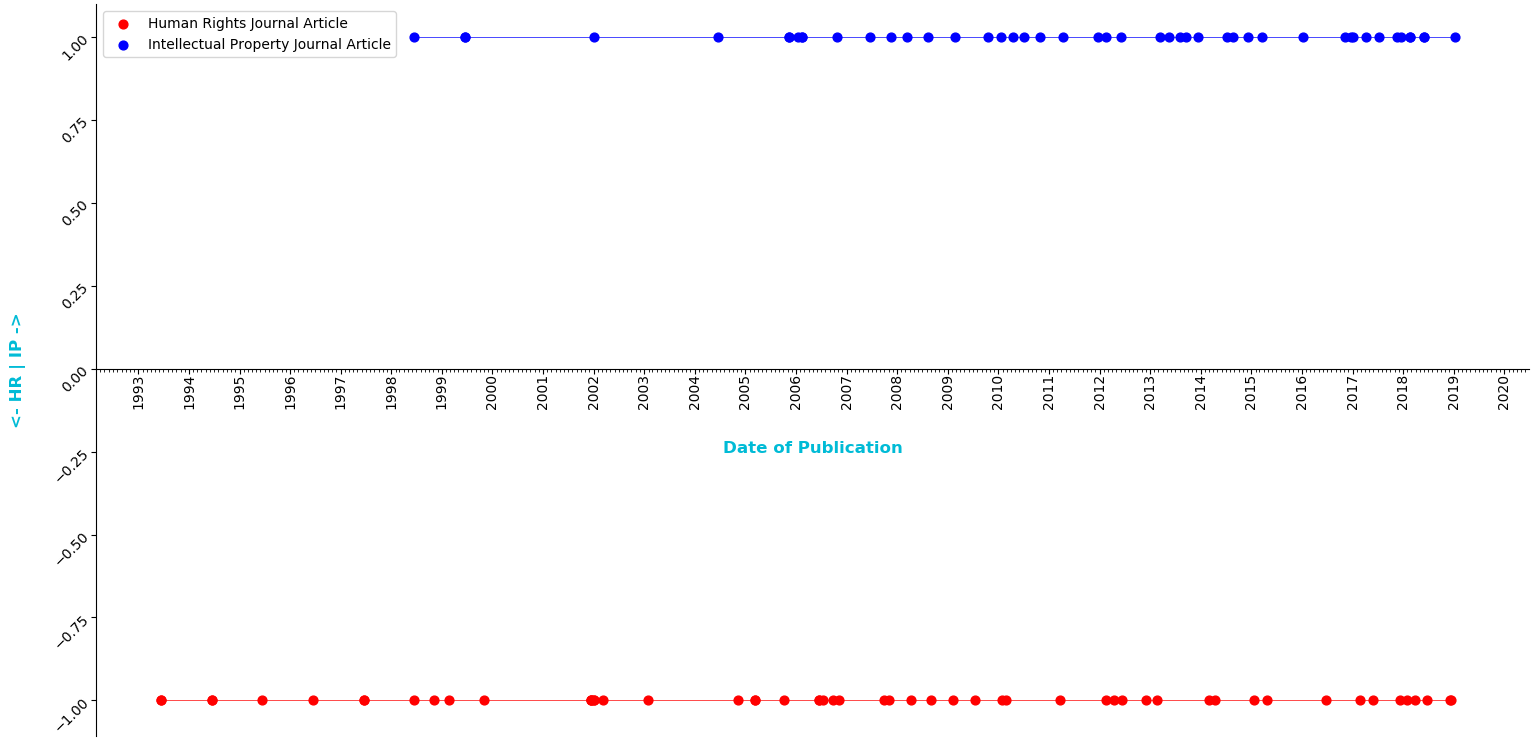
\includegraphics[width=0.9\linewidth]{resources/images/no_preprocessing.png}
        			\caption{How test documents were classified when no pre-processing was done to the text.}
        			\label{fig:no_preprocessing}
	    		\end{figure}
				
				After analysing the text, I realised that on each article there were keywords which either overtly, by stating the journal of origin, or covertly, by including metadata of a certain format, revealed the article's parent class. It appeared that the model was classifying based on the format of the document as these were the most distinguishing features, contrary to the requirement to analyse trends in language.  
				
				I analysed each different document format and identified any phrases that of this nature. They were then identified by regular expressions and removed from the text. An example of this metadata being identified were documents from the Journal of Intellectual Property Law all had some variant of ``Downloaded from http://www.academic.oup.com at the University of Bristol Library on 18 January 2019'' vertically on the right-hand side. Before pre-processing each letter was a different feature but when new lines were removed in pre-processing, they each became whole words. This meant that the word University once per page would make it clear that there was a very high chance that this document is an intellectual property document. I identified the phrase using the regular expression: \[\backslash nl\backslash n\backslash nD\backslash no\backslash nw\backslash nn[a]^+?[\backslash n ]^{7}\] and removed it. This was done with 17 expressions in total.
				
				After removing these expressions, the score of in cross-validation averaged 0.58. This suggests that the model is not much better than chance. To improve this, I performed pre-processing techniques that commonly performed well: cleaning the text of punctuation and new lines, removing features that include integers, and changing all letters to lowercase. After this, I observed that many words were being split in two, commonly if they had certain combinations of letters in them such as `ff' or `fi'. I discovered that this was to do with letters being processed by PDFs into Unicode blocks called ligatures. These could not be interpreted by pdfminer. Therefore, I identified a list of all these ligatures which included the discovery that some ligatures were converted into a code, such as `(cid:123)'. I then replaced them, and the space following them, with the individual letters' characters which they represented. 
				
				After these steps, the results were drastically improved with a cross-validation score of 0.99. This result more than suffices in terms of accuracy but I carried on to see if removing stopwords and lemmatisation would maintain the same accuracy while reducing the feature count. Lemmatisation was performed using an nltk library function. I chose lemmatisation over stemming so the origin word is more obvious should analysis be done using the processed words. nltk also has a function for removing stopwords from text but it does not let you append your own stopwords, for this reason, I implemented my own algorithm to do this. I added words to the list such as `abstract' and `references', which again could have given away what journal an article was from based on the required structure of the journal article.
				
				As can be seen in Table \ref{tab:ppres}, all results after the first set of processing methods are similarly high. There is a slight decrease when stopwords are removed, possibly because of the words indicating the journal's structure. Performing both these methods reduces the number of features by more than a factor of three. I am choosing to use all the processing methods because it has the highest score that involves removing possibly indicative but irrelevant stopwords and it has the fewest number of features.
				\begin{table}[h]
					\centering
					\begin{tabular}{l|c|c}
						\hline
						Level of Pre-processing&Number of Features&Accuracy Score\\
						\hline
						000&257604&0.579\\
						100&77669&0.991\\
						110&77356&0.981\\
						101&71464&0.992\\
						111&71363&0.984
					\end{tabular}
					\caption{The results for defferent levels of pre-processing where the three bits in the `Level of Pre-processing' column represent what pre-processing methods were performed with the most significant bit representing removing punctuation, new lines, integers and glyphs; the middle bit representing removing stopwords; and the least significant bit representing lemmatisation.}\label{tab:ppres}
				\end{table}
				
		\subsection{Trends}\label{sec:trends}
			\subsubsection{Method}
				Since the two classes are polarised, doing a line of best fit for all the data would be useless, giving a line approximately in the middle without slope. Instead, I chose to perform linear regression on each class separately. This will show how the language in each set of journals has changed over time.		
			
				The method of generating trends needs to be robust. I initially used statsmodel's ordinary least squares class but found that some extreme outliers forced this to exaggerate trends. I then switched to a robust version of ordinary least squares which appeared to be more resistant to the outliers as shown by Figure \ref{fig:regcomp}. It also improved the average p-value from 0.556 and 0.679 to 0.377 and 0.567.
				\begin{figure}
					\minipage{0.49\textwidth}
						\centering
  						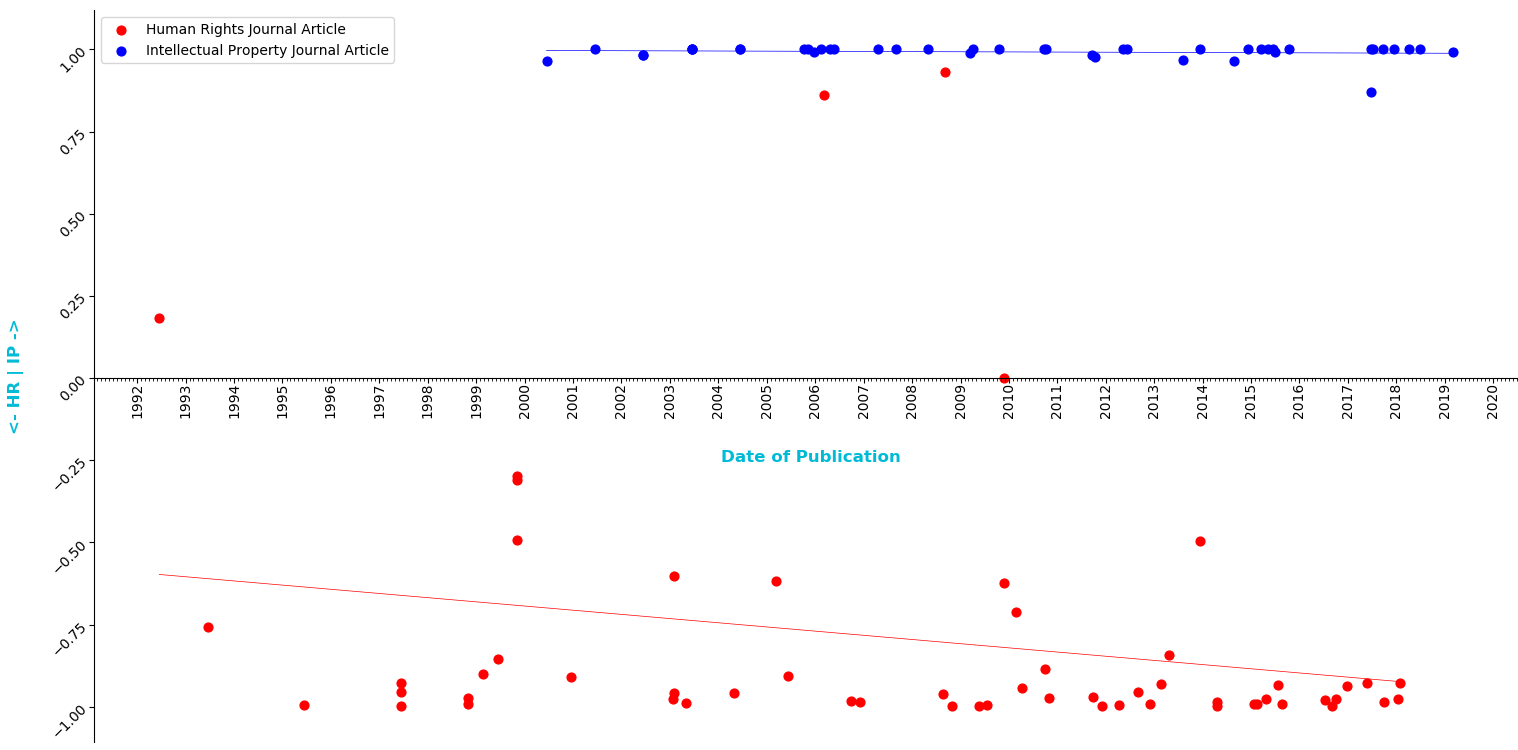
\includegraphics[width=\linewidth]{resources/images/reg_stan.png}\\
  						Trends illustrating standard least squares regression (a)
	  				\endminipage\hfill
  					\minipage{0.49\textwidth}
  						\centering
  						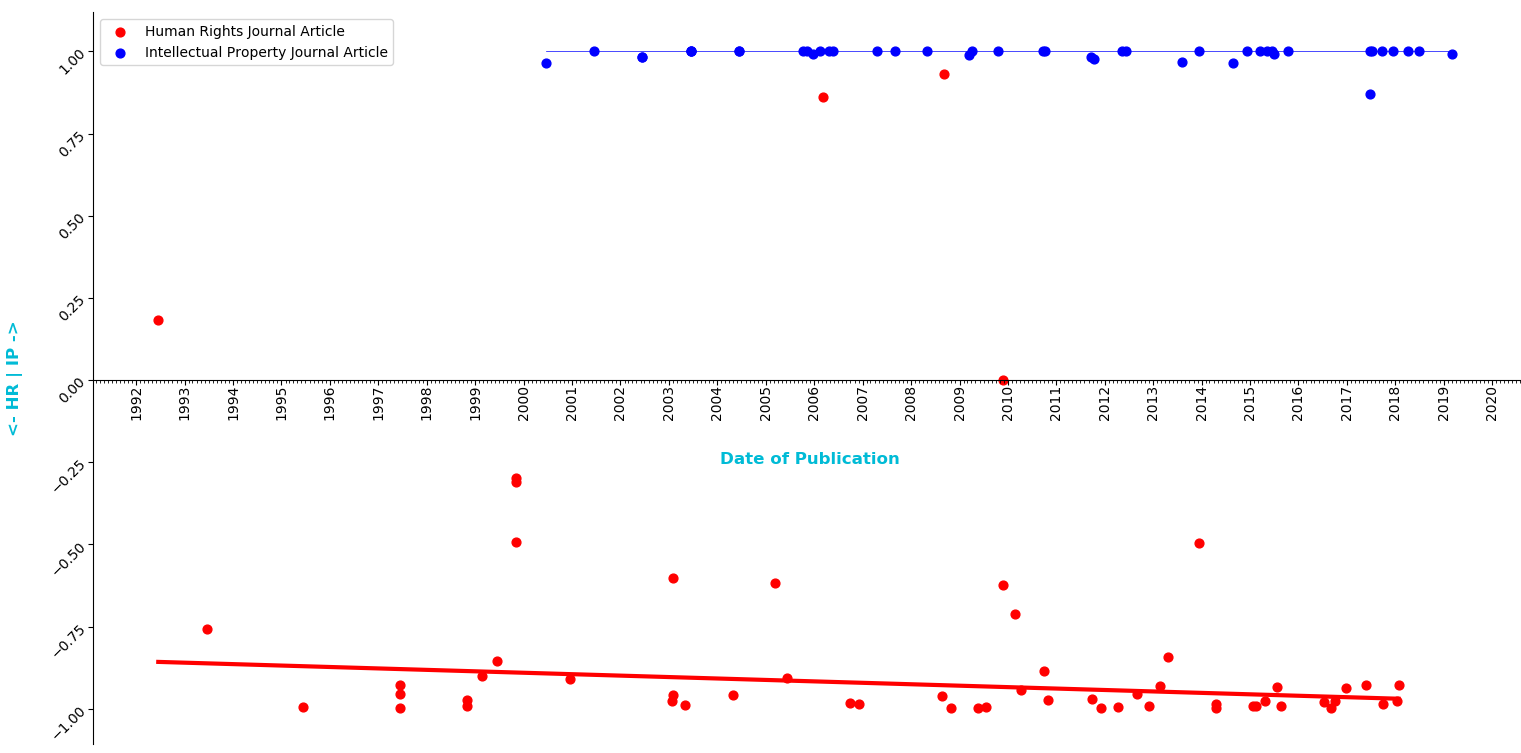
\includegraphics[width=\linewidth]{resources/images/reg_rob.png}\\
  						Trends illustrating robust least squares regression (b)
  					\endminipage\hfill\caption{The same dataset with different types of linear regression performed on it.}\label{fig:regcomp}
				\end{figure}
				
		\subsection{Human Rights-Intellectual Property Classification}\label{sec:hripimp}
			\subsubsection{Motivation}
				Here, I will look to model what a typical human rights and intellectual property document looks like respectively. I will test its accuracy on a different set of test documents and detect whether any significant trends have appeared based on these trends. In classification, we are looking for the highest possible level of accuracy to show that the model works and the lowest possible p-value in order to find a trend in the data.
			\subsubsection{Training Model}
				In my implementation, I chose to use scikitlearn's support vector machine class as it is simple and often outperforms naive Bayes. This class has an attribute that gives the probability that each document belongs to a topic, $p(hr)$ and $p(ip)$. To get a value which I will later plot, I will use a simple equation, Equation \ref{equ:hrip}.
				\begin{equation}\label{equ:hrip}
					hr\textnormal{-}ip\textnormal{ }score = p(ip) - p(hr)
				\end{equation}
			\subsubsection{Training Documents}
				Dr. Blakely thought that it may be interesting to use the treaties specified in Table \ref{tab:treaty-list} as the training documents as they are the legal basis for the fields. However, four documents turned out to be not enough to train a model. The results are fairly meaningless with a consistent score of 0.5 and no meaningful trends shown by Figure \ref{fig:train-treat}. Instead, I chose to use three-quarters of the articles in the dataset I downloaded in Subsection \ref{sec:webtotext}. This is a high enough proportion of the documents to give an accurate classification of the test documents but low enough to give the opportunity to find some statistically significant trends.	
			\begin{figure}
    			\centering
    			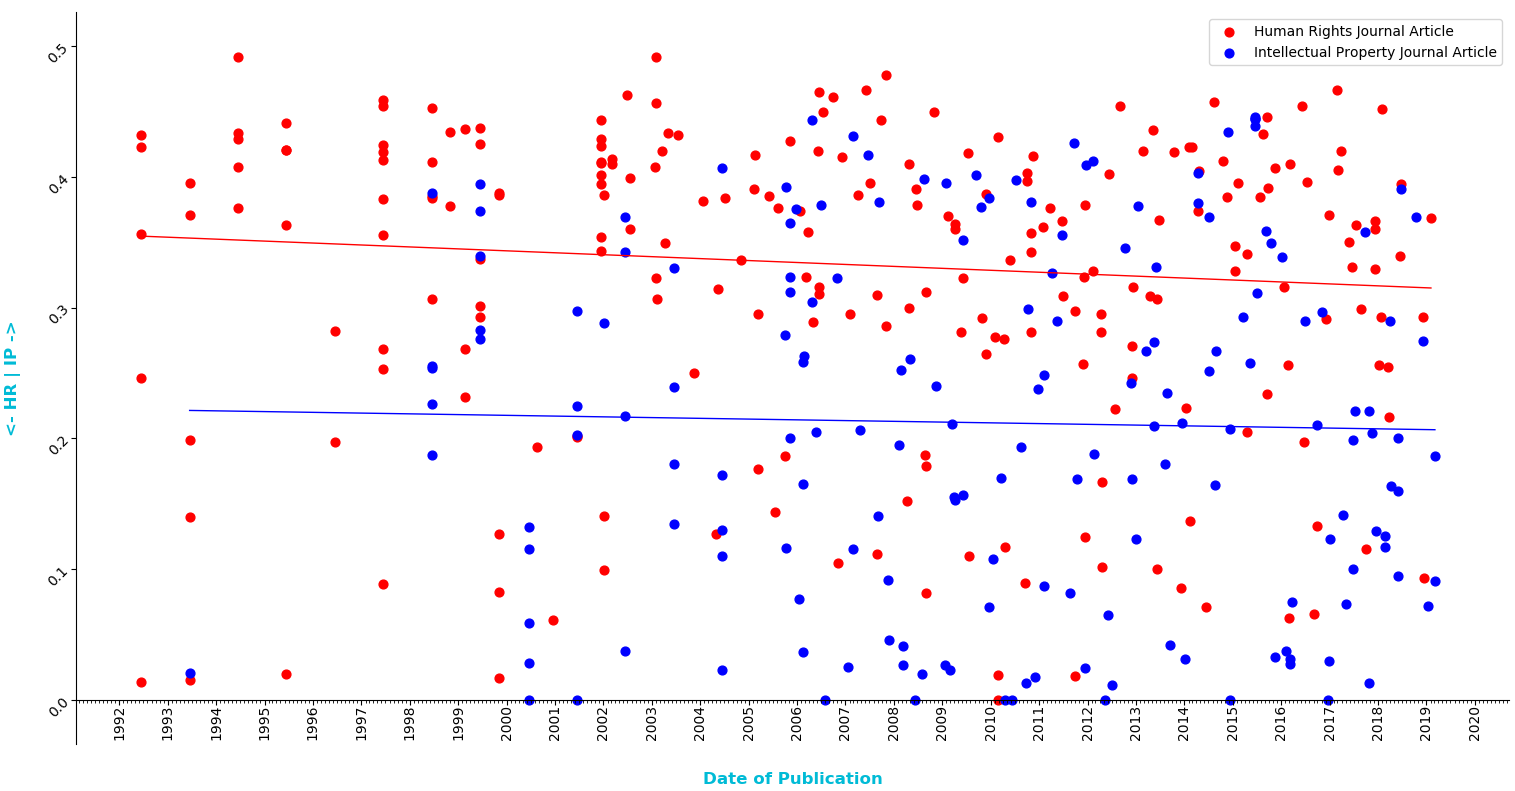
\includegraphics[width=0.9\linewidth]{resources/images/treaties_hrip.png}
    			\caption{The results of testing when using four treaty documents to train.}
    			\label{fig:train-treat}
			\end{figure}
			
			\subsubsection{Feature Count}
				I used a bag of words model for features. This involved separating each word in an article and including each unique word as a feature. 
				
				I started counting features by simply implementing an algorithm to count the number of occurrences of each term in a document. This gave a suitably high result of 0.97. However, I deemed that occurrence count might not be solely considering the language of the article. It is likely that each journal has word limits for article submission and this could be reflected in the feature count and affect classification. This can be seen by the fact that 27\% of intellectual property articles are between 4,000 and 5,000 words while only 15\% of human rights documents are. Although, the total word count is not a feature in itself, the fact that the average feature will probably lie in a certain space means that a document between these word counts would be more likely to be classified as an intellectual property document. This is another case of an attribute other than the article's language influencing classification which goes against the requirements. Using term frequency in the feature count removed this possible bias. 
			
				I implemented algorithms for four types of feature counts based on their equations given in Subsection \ref{sec:litrev-langfet}. Their results are shown in Table \ref{tab:featres}. It shows that tf-idf-cf has the highest accuracy and the lowest p-values.
				\begin{table}[h]
					\centering
					\begin{tabular}{l|c|c|c}
						\hline
						Feature Type&Average Accuracy Score&Average HR p-value&Average IP p-value\\
						\hline
						word occurrence&0.973&0.222&0.602\\
						tf&0.962&0.588&0.570\\
						idf&0.940&0.191&0.370\\
						tf-idf&0.946&0.213&0.693\\
						tf-idf-cf&0.984&0.227&0.157
					\end{tabular}
					\caption{The results for different types of features.}\label{tab:featres}
				\end{table}
			\subsubsection{Trends Found}
				On the rare occasion a statistically significant trend was detected, human rights documents began to include more typical human rights language. Cross-validation showed that this was particularly infrequent, happening once in the four folds at most, and therefore, not worth taking seriously.
	\section{User-Creator Classification}
		\subsection{Motivation}
			Here, I will look to model what a typical document which portrays the legal climate as user-benefiting as opposed to creator-benefiting and vice-versa looks like. Again, the aim of this classification is to get the highest accuracy possible with the lowest p-values to find a trend. 
		\subsection{Ground Truth}
			Unlike the human rights-intellectual property model, there is no extensive dataset for indicating whether an article is user-benefiting or creator-benefiting. Instead, Dr. Blakely supplied a list of keywords that suggested each. These are given in Table \ref{tab:keyword-list}. During my preliminary investigations, I prompted Dr. Blakely to extend her keyword lists by visualising the word occurrence count in each class of journal articles and the word occurrence count in each class of journal articles in sentences where a keyword occurs. These visualisations for intellectual property journals and creator keywords are shown in Figure \ref{fig:prelim-count}. Dr. Blakely stated she did not wish to add more words to the list.
			
			\begin{figure}
				\minipage{0.49\textwidth}
					\centering
  					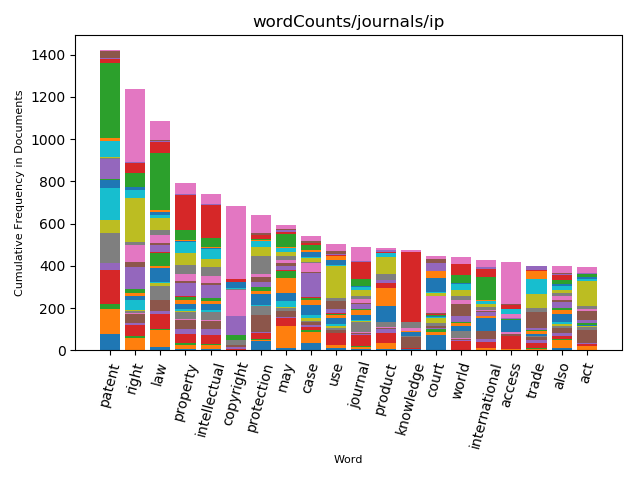
\includegraphics[width=\linewidth]{resources/images/prelim_total_count.png}\\
  					Total word counts in intellectual property articles (a)
  				\endminipage\hfill
  				\minipage{0.49\textwidth}
  					\centering
  					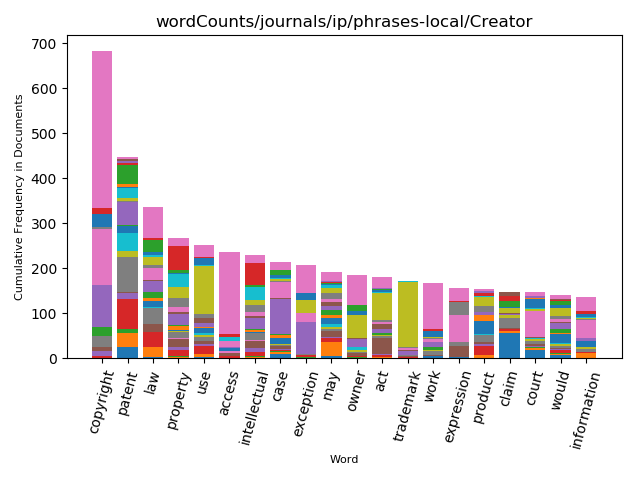
\includegraphics[width=\linewidth]{resources/images/prelim_local_count.png}\\
  					Word counts in intellectual property articles in sentences that continaed creator keywords (b)
  				\endminipage\hfill\caption{The visualisation of word counts as part of preliminary investigations.}\label{fig:prelim-count}
			\end{figure}
			
			In order to evaluate my model, I assigned my own document document-by-document ground truth to 20 randomly selected documents since Dr. Blakely was not available. This must be taken with quite the pinch of salt since my experience in this domain does not stretch beyond this project. Also, since the model does not train on documents itself, cross-validation was not used for evaluation for this model, the same 20 documents are repeatedly checked to see if their prediction matches ground truth. In reality, the small test set and that curated by someone who knows little about the fields, indicates that the evaluations that took place in this section were unreliable.
		\subsection{Method}
			I attempted to use a lexicon-based system to give each document a score on how it scales based on a creator score and a user score as shown in Equation \ref{equ:user-creator}, where positive scores are classified as creator-benefiting and negative scores as user-benefiting.                              
			\begin{equation}\label{equ:user-creator}
				user\textnormal{-}creator\textnormal{ }score = creatorscore - userscore
			\end{equation}
			I began this by considering every sentence as indicating an independent sentiment on whether the legal climate was user-benefiting or creator-benefiting. I then assigned $creatorscore$ as the proportion of sentences that included a creator keyword and treated $userscore$. This resulted in a balanced accuracy score of 0.75. Because the keywords chosen for creator-benefiting were more common than the keywords for user-benefiting, this resulted in a large proportion of documents being classified as creator-benefiting. The average p-value upon cross-validation was 0.196. 
			
			This model's main weakness was that it did not really capture the sentiment since it ignored negators which completely changed the meaning of the sentence. For example, the clauses “this means that the user will have access” and “this means that the user will not have access” are both scored as benefiting the user when the latter clause clearly does not benefit the user. My next approach, therefore, was to extend the model to consider the sentiment of each sentence. This included creating five lists based on Mandal and Gupta's\cite{lexicon_sentiments_mandal}: comparative positive, comparative negative, superlative positive, superlative negative and negators. I implemented an algorithm that assigned a $creatorscore$ of 1 if the sentence contained a word from the creator keyword list. The algorithm then checks for any words in the above lists. The current score is added to if a positive word comes up and then subtracted from if a negative word comes up. The scalar used is 0.65 for a superlative and 0.35 for a comparative. The score is multiplied by -1 if a negator word comes up. So, for example, the sentence ``What we can do is carefully study the development of patent pooling regulations in other countries and implement the most successful models for protecting IP rights and promoting fair competition'' now receives a $creatorscore$ of 1.65 because of the word patent which is enhanced by the word most. I then divided by the number of sentences in the article. The equivalent is done with $userscore$.
			
			This method did not actually cause any classification changes as the lists were not extensive enough. It also raised the average p-value in cross-validation to 0.465, making statistically significant trends very rare. Since this method was not developed enough, it produced no trends over cross-validation of p-values and there was no way to be sure this model was accurate since my evaluation method was poor, I decided to not use this option. I chose to use the simpler option as it's clearer what it represents.
			
			Both these methods were weak in that the keyword lists contained some of the same words, leading to sentences containing keywords from both lists cancelled out when they are likely to have higher importance than usual. This can be 
		\subsubsection{Trends Found}
			Trends were found approximately half the time with the chosen model. As this model had not been properly evaluated for accuracy, however, I fully explained how the model worked to Dr. Blakely and explained that proper evaluations would need to be done before any conclusions were drawn.
	\section{Visualisation}
		\subsection{Evaluation}
			\subsubsection{Motivation}
			    The result of the natural language processing is a collection of probabilities, scores and gradients. This would mean very little to the average law academic without explanation. The purpose of the visualisation is to explain these numbers so anyone can understand them with as little comprehension as possible. Simply plotting each test document's date of publication on the x-axis against the results of its human rights-intellectual property classifications on the y-axis against the results of its user-creator classifications on the z-axis with no further configuration of the visualisation gives Figure \ref{fig:blank-vis}. This was plotted using Python's `matplotlib' library. The `Axes3D' class allows the user to change the angle of the visualisation using their mouse.
			    
			    A successful evaluation method will convert Figure \ref{fig:blank-vis} into the perfect visualisation for the target audience in minimal time. This will be possible if the evaluation method allows for informative communication and allows visualisations to be compared. It is worth noting that the visualisations in this section are not shown in chronological order and are simply placed in the order which best shows the effect of the change being discussed. It is also worth noting that each visualisation does not necessarily show the same data plotted. It should be apparent that the changes discussed apply to the task whatever combination of data is plotted.
				\begin{figure}
    				\centering
    				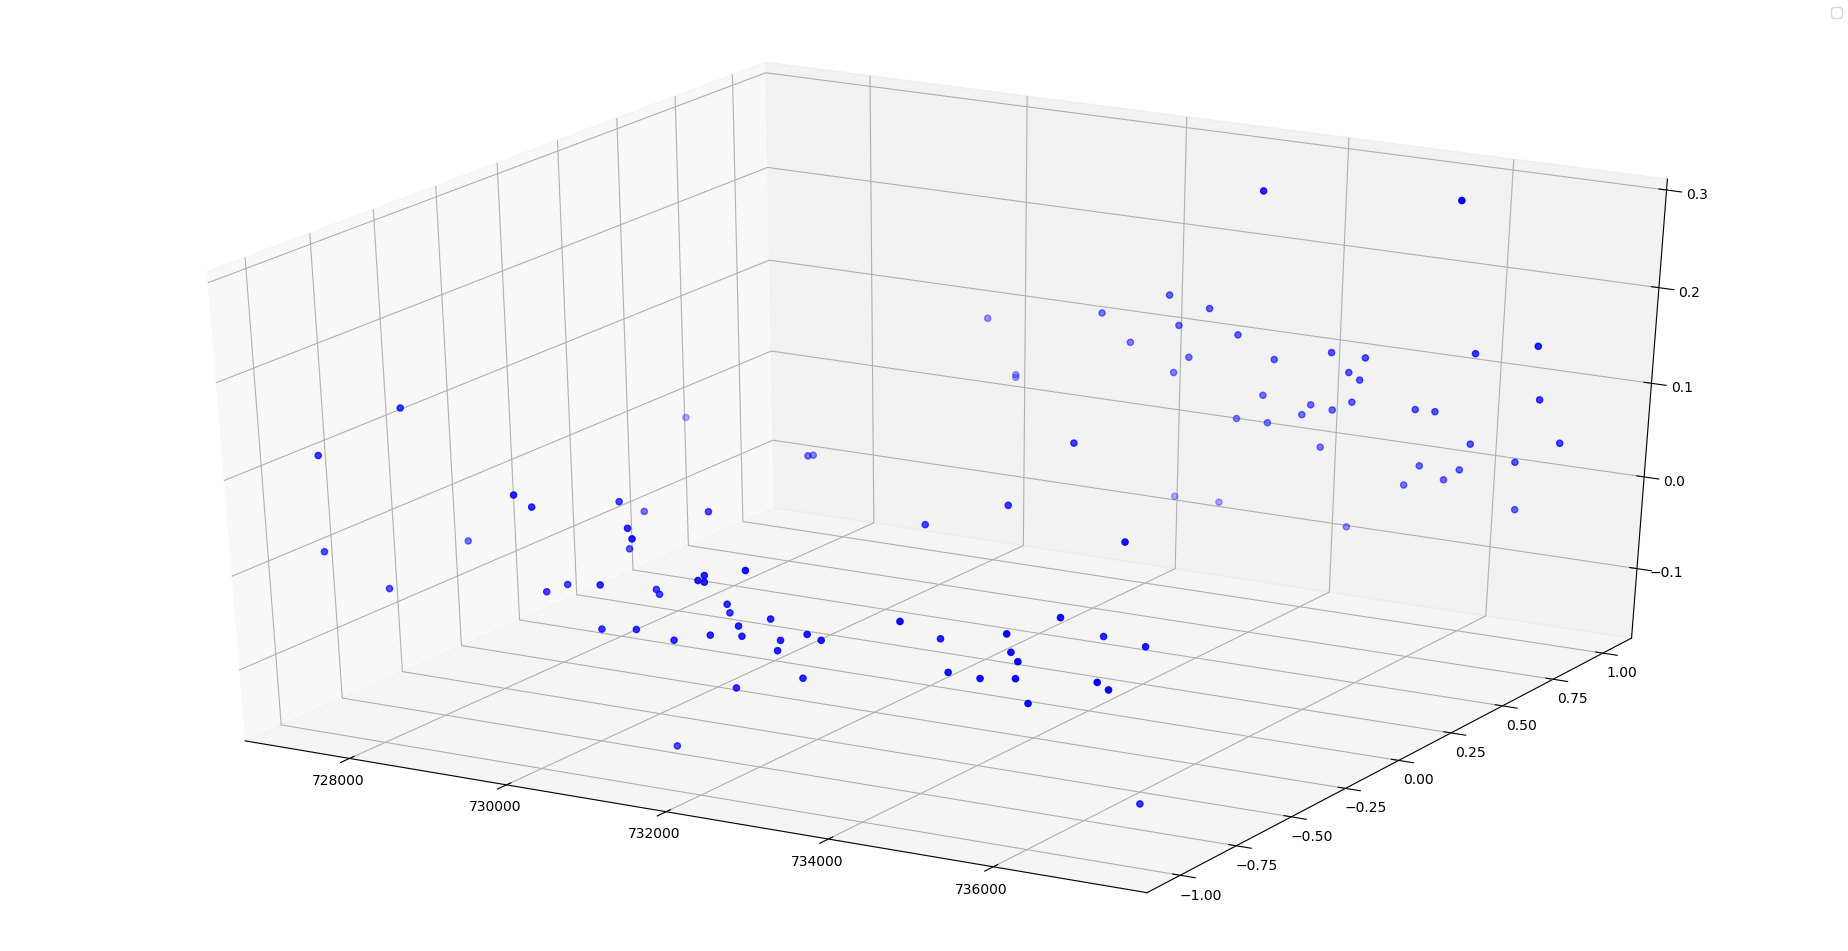
\includegraphics[width=0.9\linewidth]{resources/images/blank_vis.png}
    				\caption{Documents plotted with no further configuration.}
    				\label{fig:blank-vis}
				\end{figure}
				
			\subsubsection{Criteria}
				Visualisations were evaluated based on the following criteria:
				\begin{enumerate}				
					\item The visualisation and its axes' meanings are self-explanatory;
					\item It is clear where a point lies on the visualisation's axes;
					\item The visualisation has all the possible information that is desired by the audience;
					\item The visualisation clearly indicates any trends deduced by the models;
					\item The visualisation is aesthetically pleasing.					
				\end{enumerate}
				For ease of notation, a criteria will be referred to as `Criteria $n$' where $n$ is the number it has been given above.
				
				I evaluated the visualisation iteratively with Dr. Blakely and my dissertation tutor, Dr. Mowbray throughout to guide the process of constructing the visualisation. A Likert scale was be used to quantify results so they can be compared. I chose this as opposed to a continuous scale as a continuous scale may not have been defined enough and may have left inconsistencies in answers. The Likert scale was in regards to each of the five statements above and asked the user to select a statement from one to five where one represented ``Strongly Disagree'' and five represented ``Strongly Agree''. This allowed me to compare criteria so I knew where improvement should be prioritised. I also requested comments after each of the statements for an explanation of why the selected answer was given so I would know where to improve on each criteria.
		\subsection{Point Location}
			Figure \ref{fig:3d-vis} shows a lone 3D visualisation, which is what Dr. Blakely suggested. To represent a 3D space on a 2D screen, matplotlib uses luminance to portray depth. The fainter a point is, the further away it is. Dr. Mowbray disagreed with Criteria 2 as she thought this was not immediately clear enough.			
			\begin{figure}
    			\centering
    			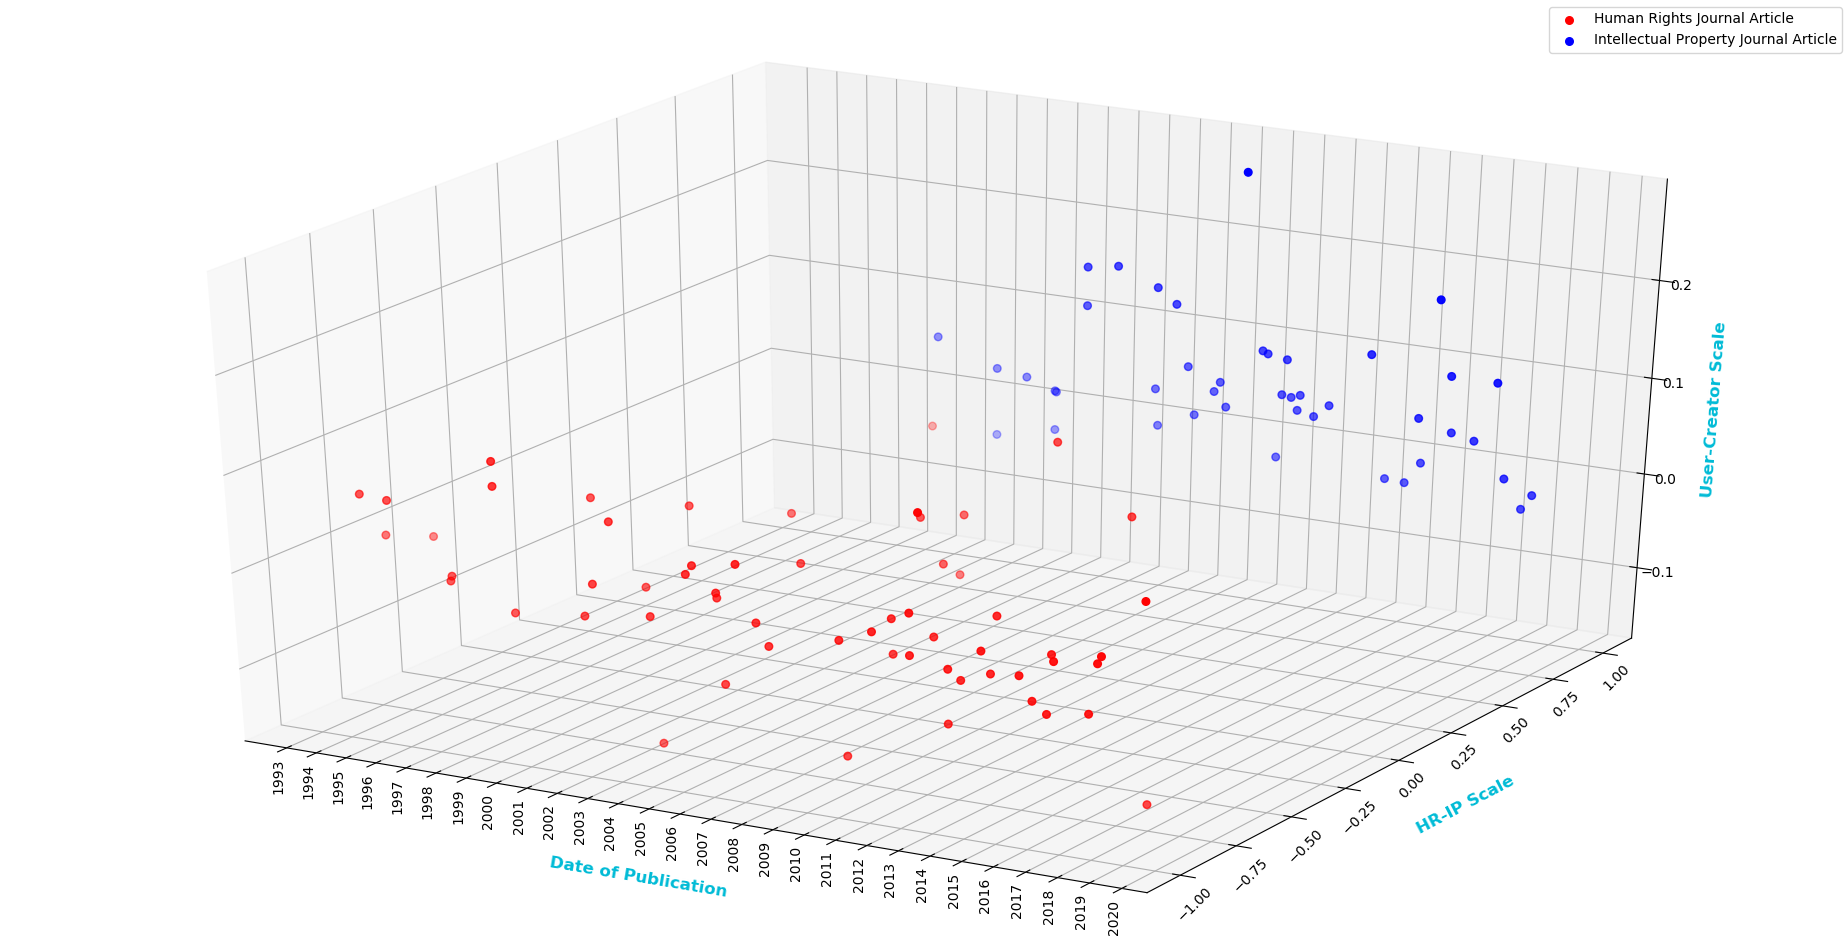
\includegraphics[width=0.9\linewidth]{resources/images/3d_points.png}
    			\caption{A visualisation advanced from Figure \ref{fig:blank-vis}.}
    			\label{fig:3d-vis}
			\end{figure}

			A 3D solution to this problem is particularly hard to find because we are limited to 2D screens. This led to the idea that there could be additional 2D axes to compare each of the three axes individually. This would allow for clearer point location and trend identification as can be seen in Figure \ref{fig:hr-ip}. The other two combinations are shown by Figure \ref{fig:trend-bold} and Figure \ref{fig:2d-arrow}. These additions prompted Dr. Mowbray to strongly agree with Criteria 2.
			\begin{figure}
    			\centering
    			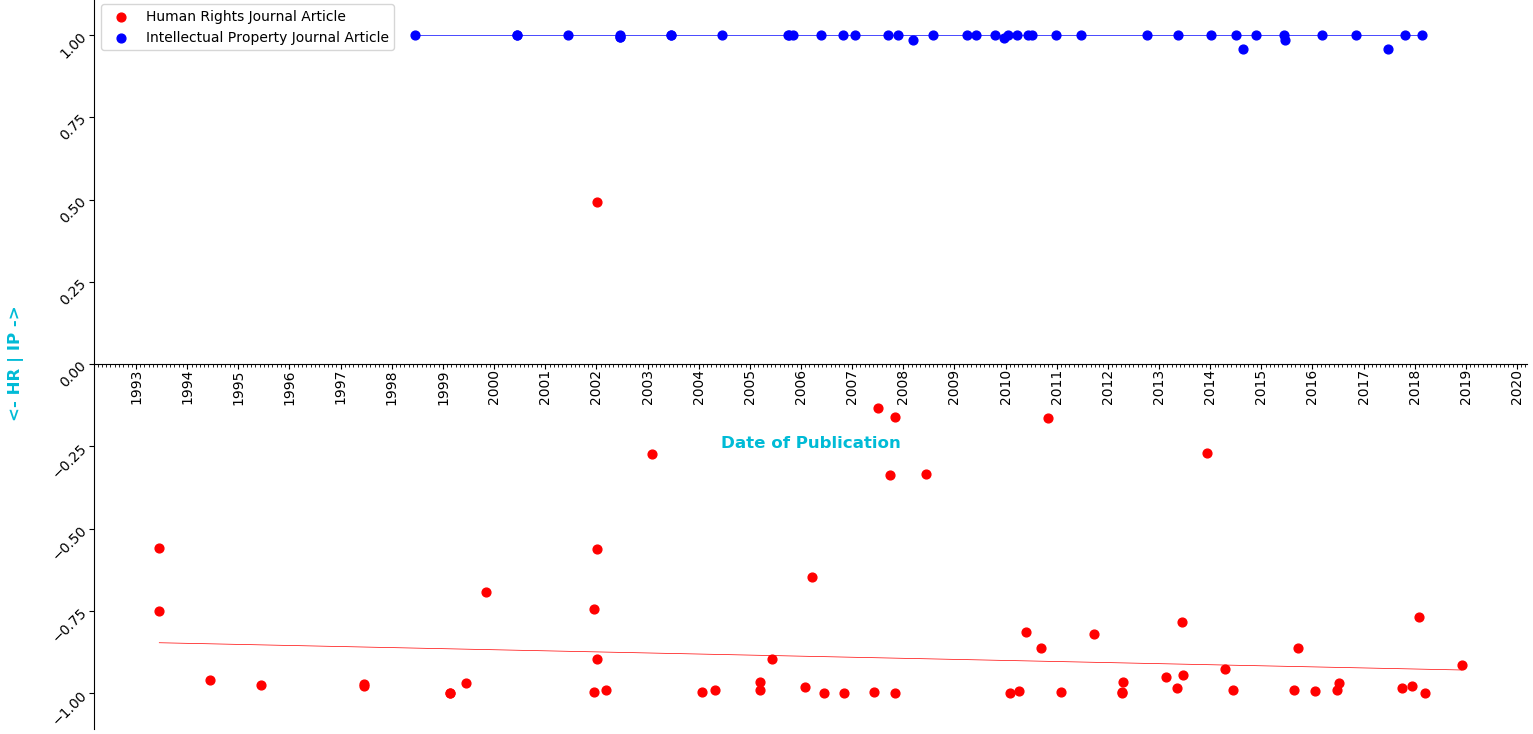
\includegraphics[width=0.9\linewidth]{resources/images/hr_ip.png}
    			\caption{A 2D visualisation of human rights-intellectual property plotted against time.}
    			\label{fig:hr-ip}
			\end{figure}
			
		\subsection{Identifying Classes}\label{fig:gtpc}
			In order to see trends in each different category, it must be immediately obvious which documents belong to which journal category. I chose the preattentive feature, colour, to distinguish between human rights journals, coloured in red, and intellectual property journals, coloured in blue, as shown in Figure \ref{fig:3d-vis}. As well as making it easy to identify trends, anomalies become particularly obvious due to the combination of preattentive features of colour and proximity. If a red point is a large distance from other points then it is obvious this is an anomaly.
			
			Initially, the 2D visualisations had their axes placed left and bottom as default as shown in Figure \ref{fig:2d-axes-out}. Where possible, I moved the axes to the zero point in the other axes. This made the most of the Gestalt principle of enclosure as the axes now enclose all points based on their predicted classification. In Figure \ref{fig:hr-ip}, it can be seen that one document has been classified incorrectly as it is below the x-axis like the rest of the red points.
			\begin{figure}
    			\centering
    			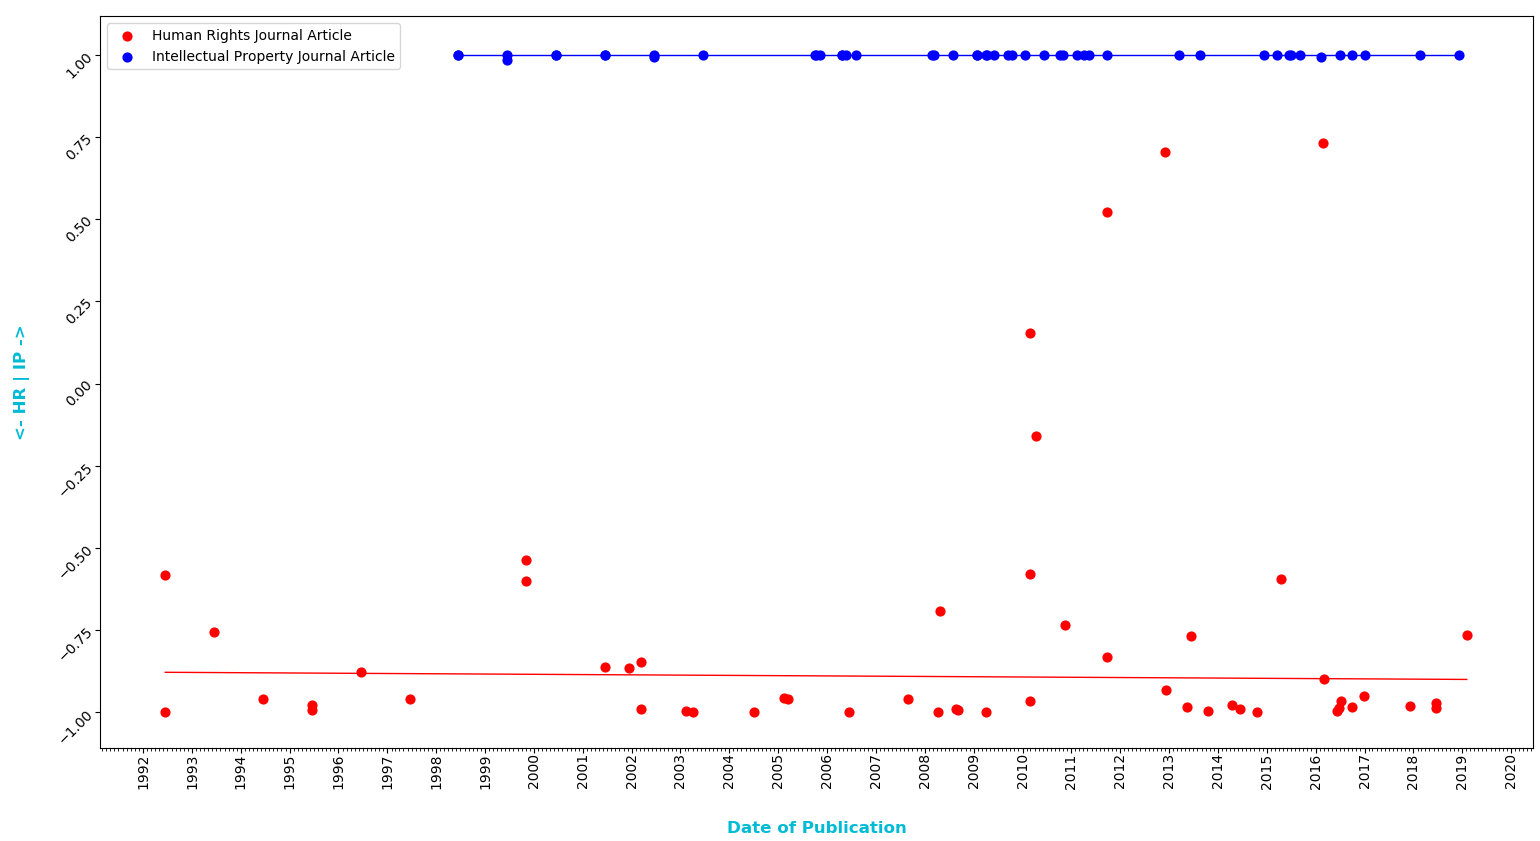
\includegraphics[width=0.9\linewidth]{resources/images/2d_axes_out.png}
    			\caption{A 2D visualisation with its axes at the left and bottom, the default positions.}
    			\label{fig:2d-axes-out}
			\end{figure}
			
		\subsection{Labelling}\label{sec:lab}
			Initially, Dr. Mowbray disagreed with Criteria 1. She commented that the visualisation was not self-explanatory because it was not clear what the points represented as the legend labelled blue points with `Intellectual Property' and red points with `Human Rights' which could refer to a number of things. To rectify this, I changed the labels to `Ìntellectual Property Journal Article' and `Human Rights Journal Article' respectively. Dr. Mowbray also commented that it was not clear what the x-axis represented as the x-axis was solely labelled with `Time' and this was not clear enough as it could refer to any number of things regarding a document. I rectified this by changing the label to `Date of Publication'. Upon these changes, Dr. Mowbray neither agreed nor disagreed with Criteria 1.
			
			Dr. Mowbray still did not agree with Criteria 1 because it was not immediately clear which end of the y and z-axes represented which class as seen in Figure \ref{fig:2d-label}. 
			\begin{figure}
    			\centering
    			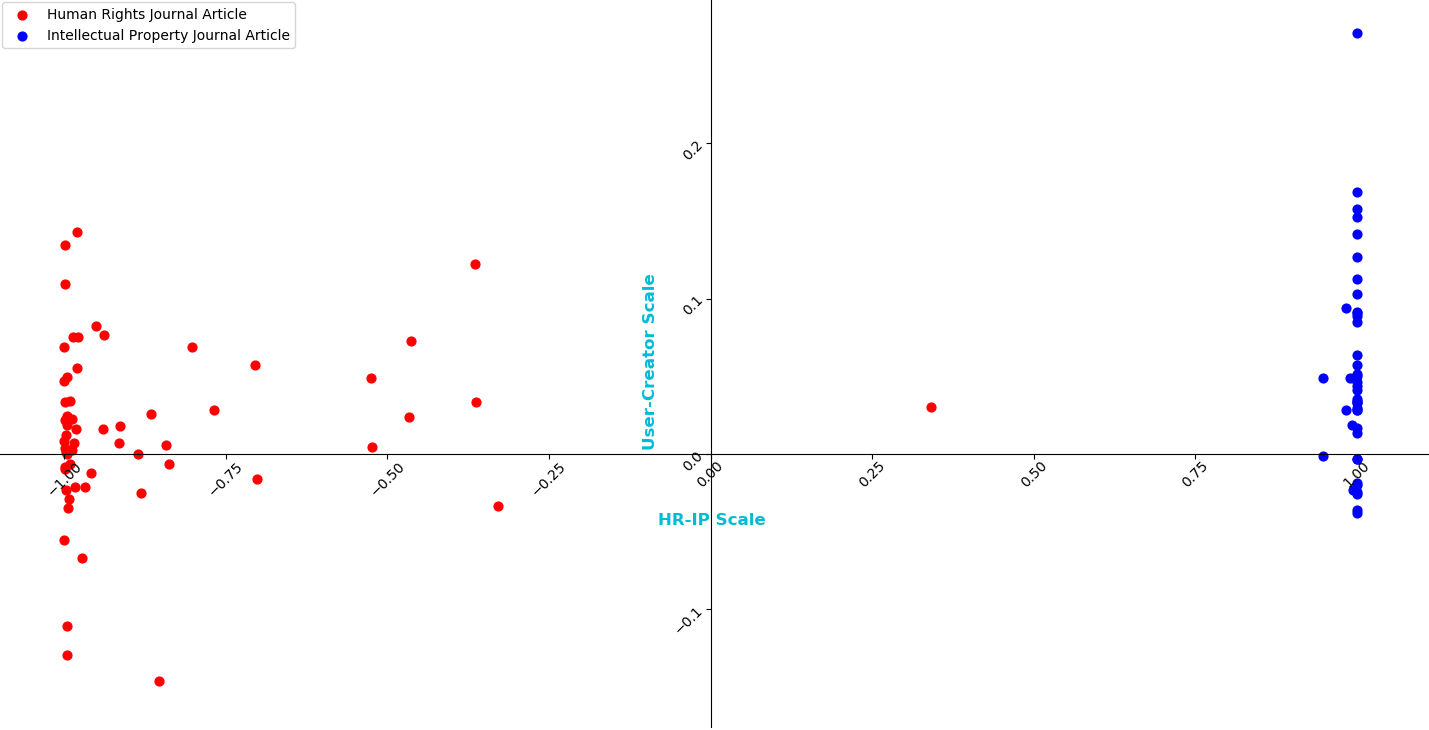
\includegraphics[width=0.9\linewidth]{resources/images/2d_label.png}
    			\caption{A 2D visualisation with basic axes labels.}
    			\label{fig:2d-label}
			\end{figure}

			To solve this, I changed the axes, `HR-IP Scale' and `Ùser-Creator Scale' to \texttt{`<- HR | IP ->'} and \texttt{`<- User | Creator ->'} respectively so the arrows were pointing in the direction that their class was represented by. This is shown in Figure \ref{fig:2d-arrow}. 
			\begin{figure}
    			\centering
    			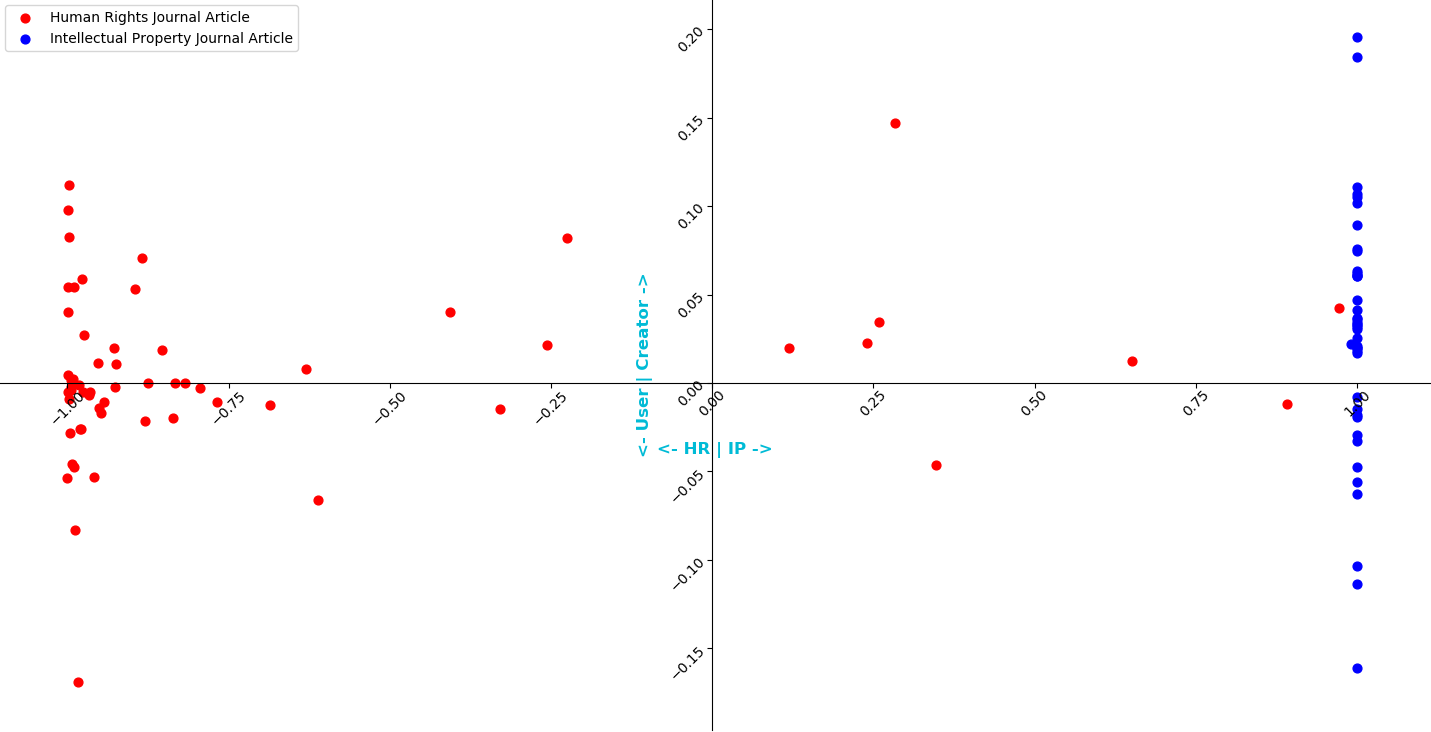
\includegraphics[width=0.9\linewidth]{resources/images/2d_arrow.png}
    			\caption{A 2D visualisation with arrows in axes labels.}
    			\label{fig:2d-arrow}
			\end{figure}	
						
			I then attempted to apply the same label change to the 3D visualisation. This was flawed because the label started off pointing the right way, shown by Figure \ref{fig:axis-switch}a but when the axes flip on the user's command, the labels do not flip causing the `HR' arrow to be pointing at the intellectual property side of the visualisation and vice versa, shown by Figure \ref{fig:axis-switch}b. This could have caused false conclusions being made based on the visualisations so had to be avoided.
			\begin{figure}
				\minipage{0.49\textwidth}
					\centering
  					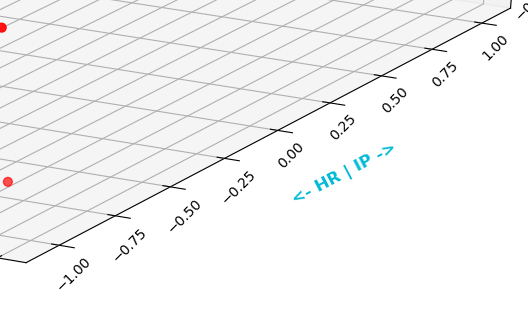
\includegraphics[width=\linewidth]{resources/images/3d_point_correct.png}\\
  					Axes label pointing the right way (a)
  				\endminipage\hfill
  				\minipage{0.49\textwidth}
  					\centering
  					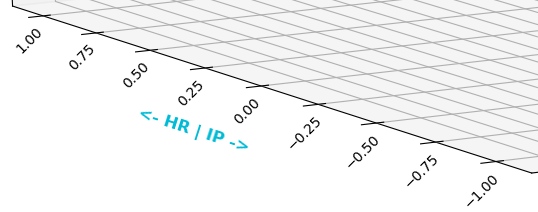
\includegraphics[width=\linewidth]{resources/images/3d_point_incorrect.png}\\
  					\vspace{1.5cm}
  					Axes label pointing the wrong way (b)
  				\endminipage\hfill\caption{The same axes labels as Figure \ref{fig:2d-arrow} on 3D axes.}\label{fig:axis-switch}
			\end{figure}
			
			As a solution, I annotated the graph at the beginning of the x-axis to indicate at which sides of the graph indicate which classes, as shown in Figure \ref{fig:3d-float}. This made it clear which end of the axes meant which class and also slightly improves the user's ability to locate where points are. 
			\begin{figure}
    			\centering
    			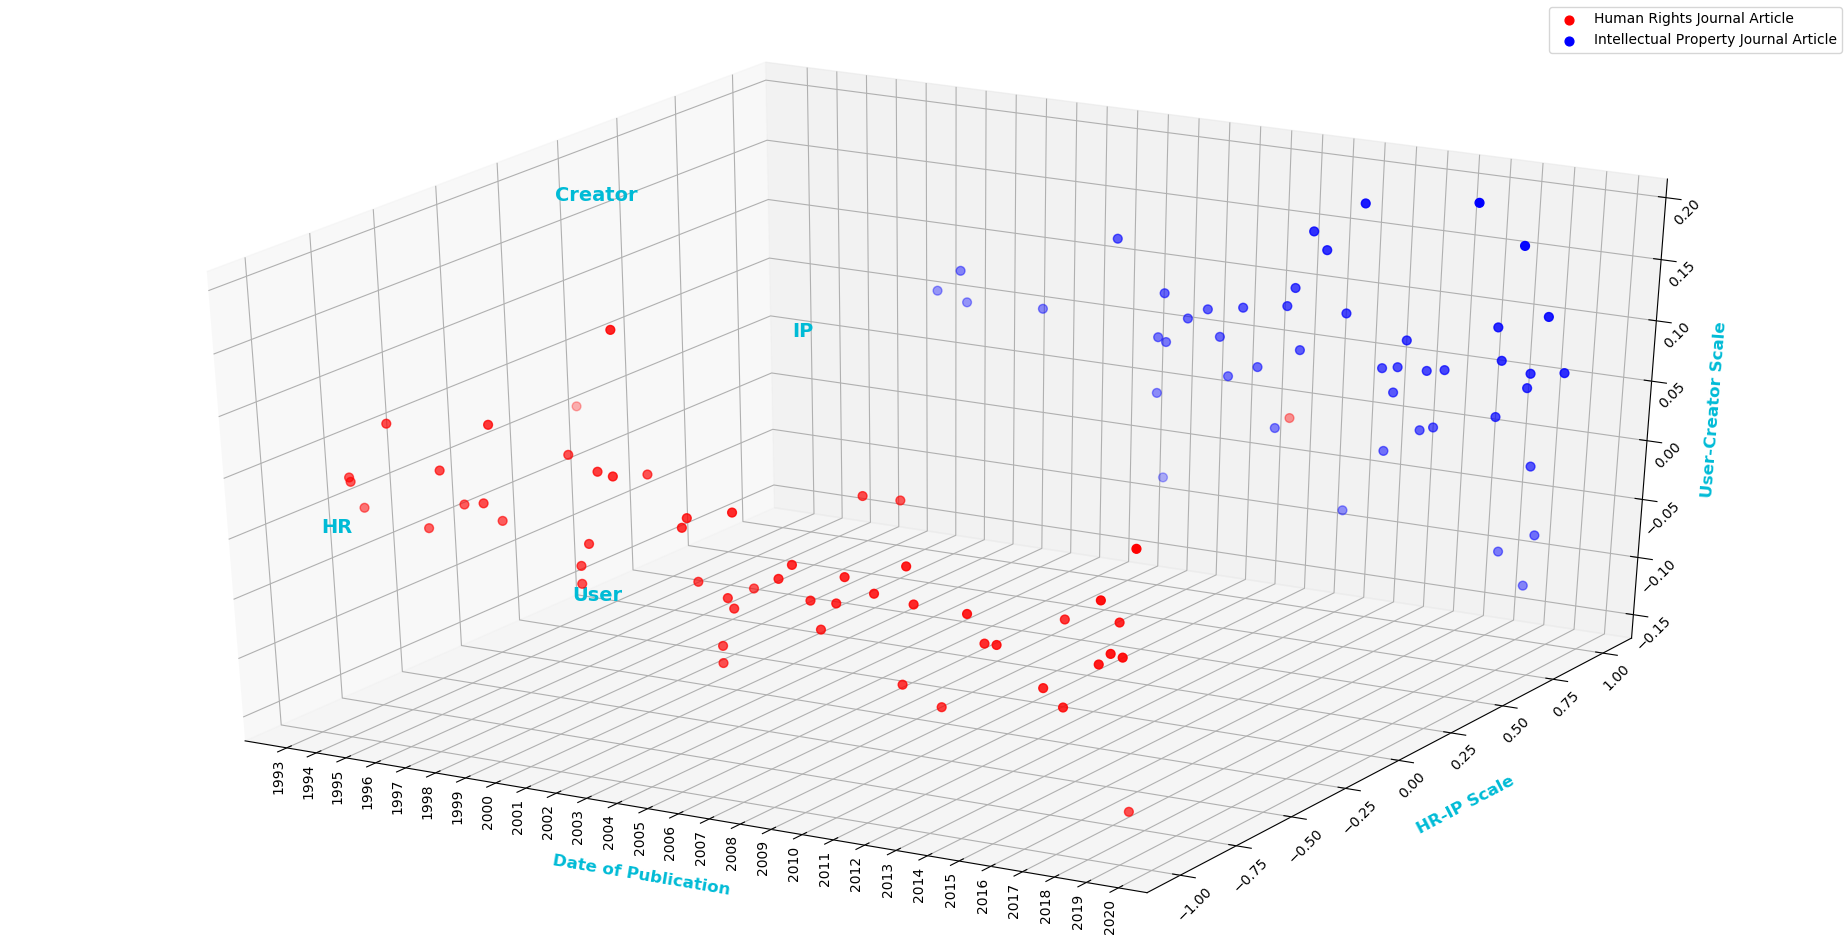
\includegraphics[width=0.9\linewidth]{resources/images/3d_float_label.png}
    			\caption{The 3D visuaisation from Figure \ref{fig:3d-vis} with annotations to make axis polarity clear.}
    			\label{fig:3d-float}
			\end{figure}

			In the interest of consistency, I attempted the same solution for 2D graphs but this was considerably worse than the solution found in Figure \ref{fig:2d-float} because the labels were covered up by points due to the polarised nature of the dataset. Therefore, I chose to stick to the original solution.
			\begin{figure}
    			\centering
    			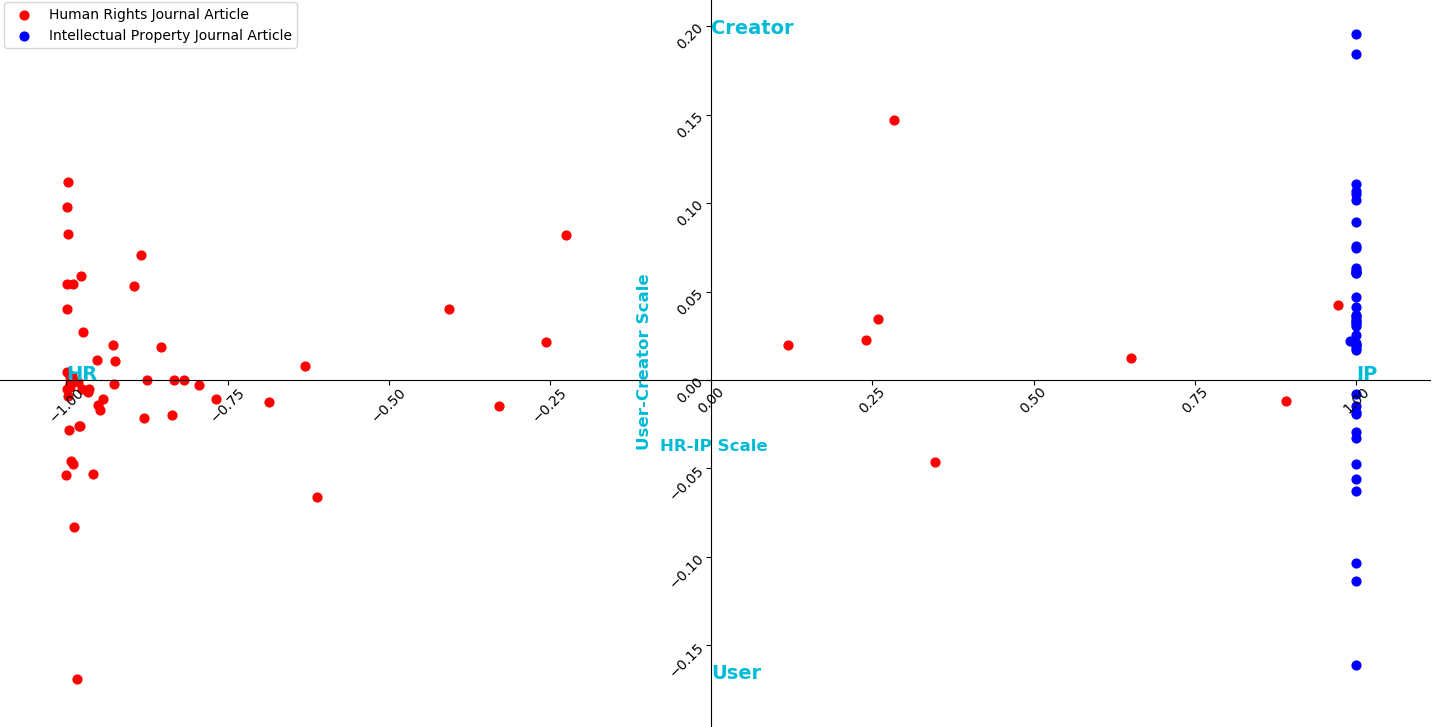
\includegraphics[width=0.9\linewidth]{resources/images/2d_float_label.png}
    			\caption{2D visualisation with axis polarity labelled by annotations.}
    			\label{fig:2d-float}
			\end{figure}
			
		\subsection{Trends}
			Initially, trends had to be deduced by eye. This could be particularly difficult when you are trying to deduce the trend for a subset of the data points and the other data points are interspersed within the subset as in Figure \ref{fig:trend-none}. In order to make trends more obvious, I plotted the results of the linear regression from Subsection \ref{sec:trends} by finding the y-values for a set of x-values based on the result's gradient and y-intercept as in Figure \ref{fig:trend-not-bold}. This visualisation could be deceiving to users as a line that is statistically significant is presented as significant as one that is not. For this reason, I made lines that are found to be statistically significant, six times thicker than ones that are not as in Figure \ref{fig:trend-bold}. I chose to keep the line that represented the non-statistically significant trend but make it half as thick as it originally was. The thinness shows its lack of significance but its existence allows the user to investigate further if they find a detail, such as the direction of the trend, interesting.
			\begin{figure}
    			\centering
    			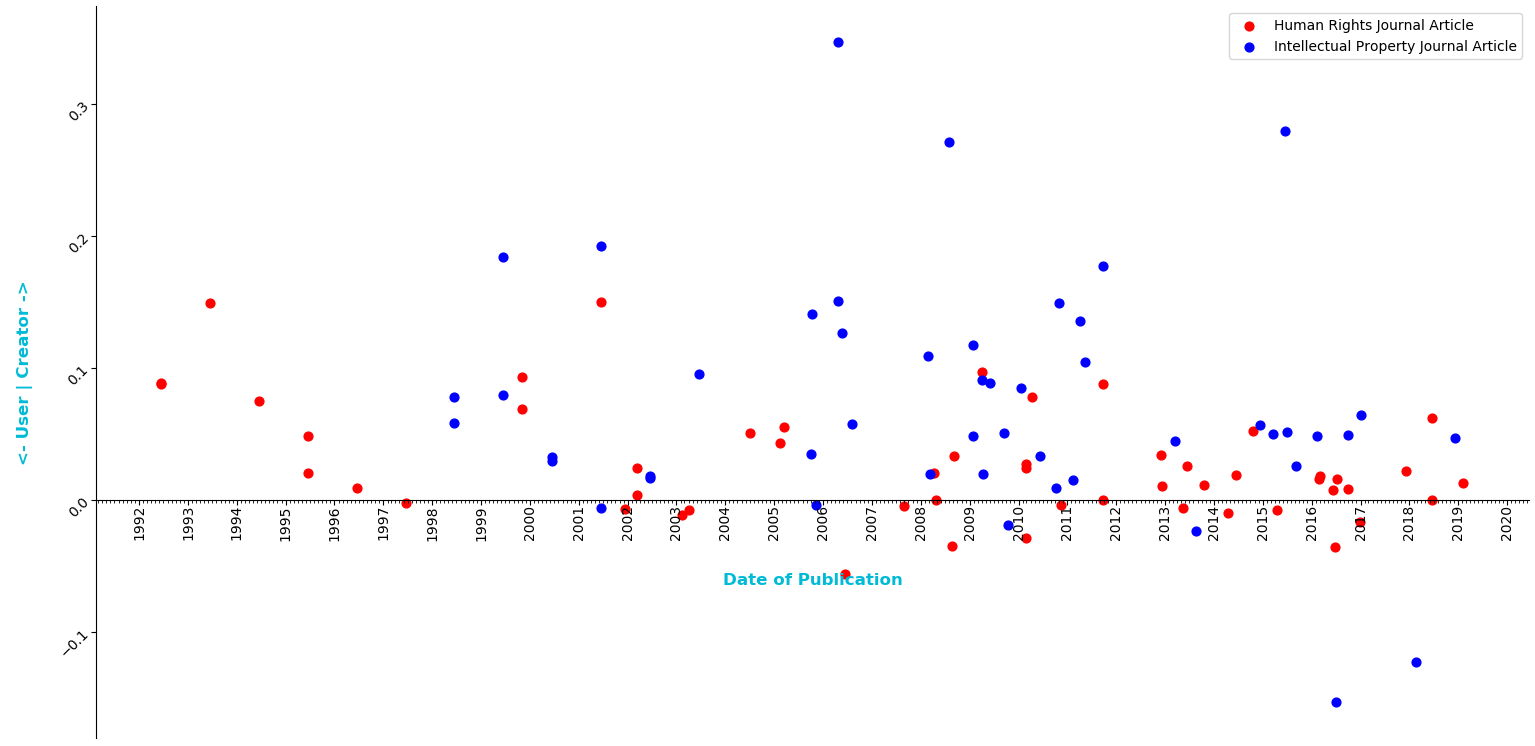
\includegraphics[width=0.9\linewidth]{resources/images/trend_none.png}
    			\caption{A 2D visualisation without any trend lines.}
    			\label{fig:trend-none}
			\end{figure}
			\begin{figure}
    			\centering
    			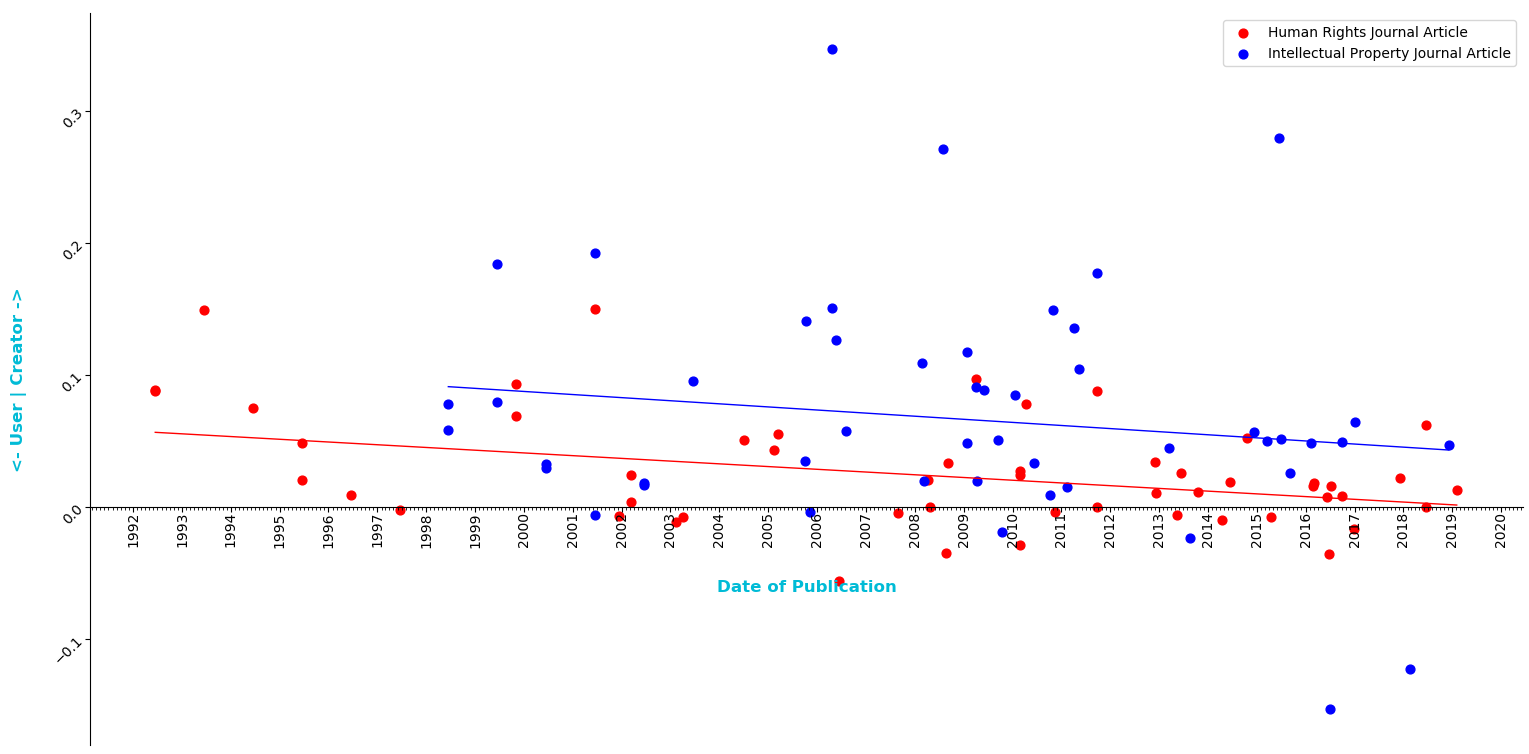
\includegraphics[width=0.9\linewidth]{resources/images/trend_not_bold.png}
    			\caption{A 2D visualisation with standard trend lines.}
    			\label{fig:trend-not-bold}
			\end{figure}
			\begin{figure}
    			\centering
    			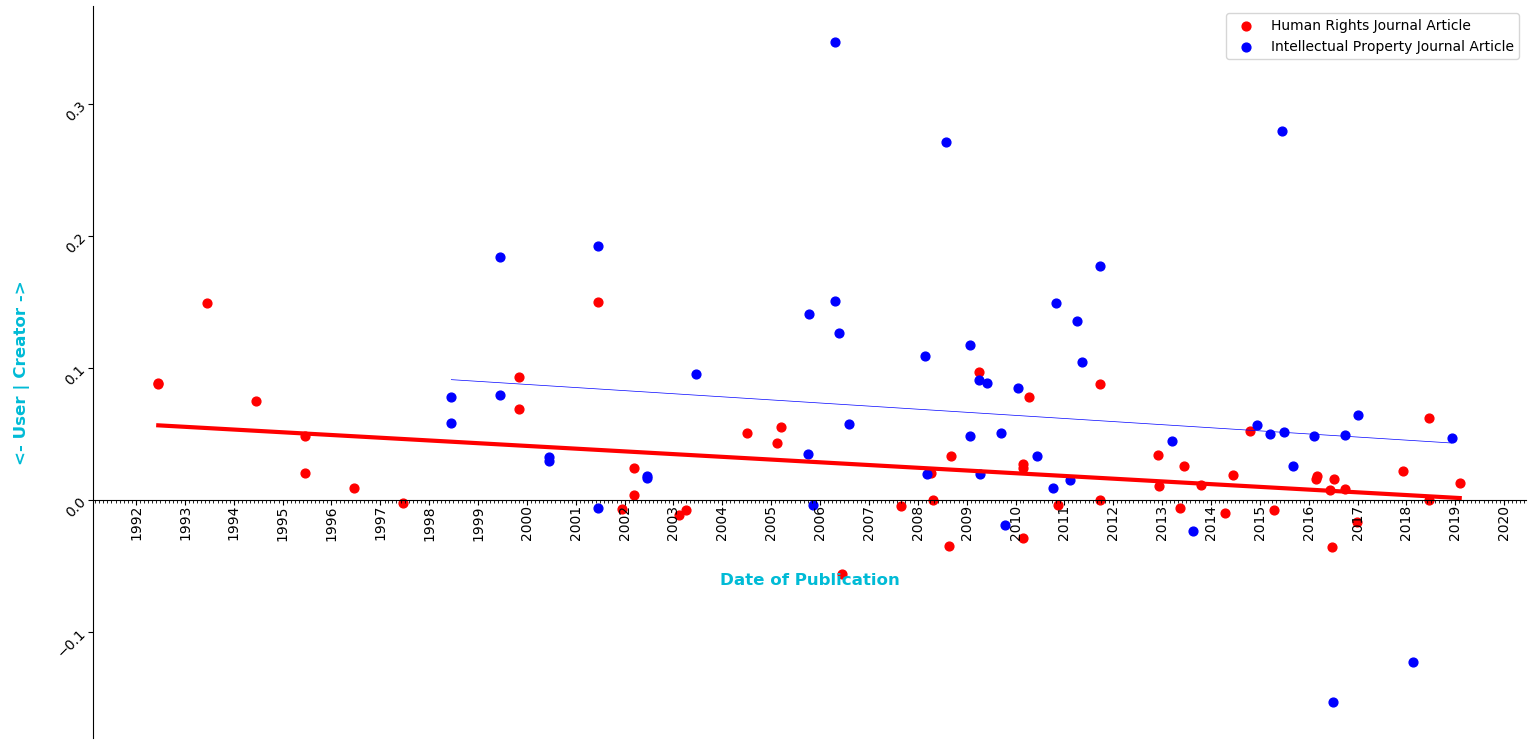
\includegraphics[width=0.9\linewidth]{resources/images/trend_bold.png}
    			\caption{A 2D visualisation with bold trend lines if statistically significant, thin if not.}
    			\label{fig:trend-bold}
			\end{figure}
			
		\subsection{Investigating Documents}
			Anomalies are important as they show where the two fields intersect most. The fact there is an anomaly is not too interesting without being able to understand why. Initially, there was no way of finding out about which point represented which document. I changed this by adding an event listener to listen out for clicks. If a click occurred somewhere a point was, the details of that point appear as in Figure \ref{fig:anomaly}. Now any anomalies can be investigated to further understanding of where the fields intersect most.
			\begin{figure}
    			\centering
    			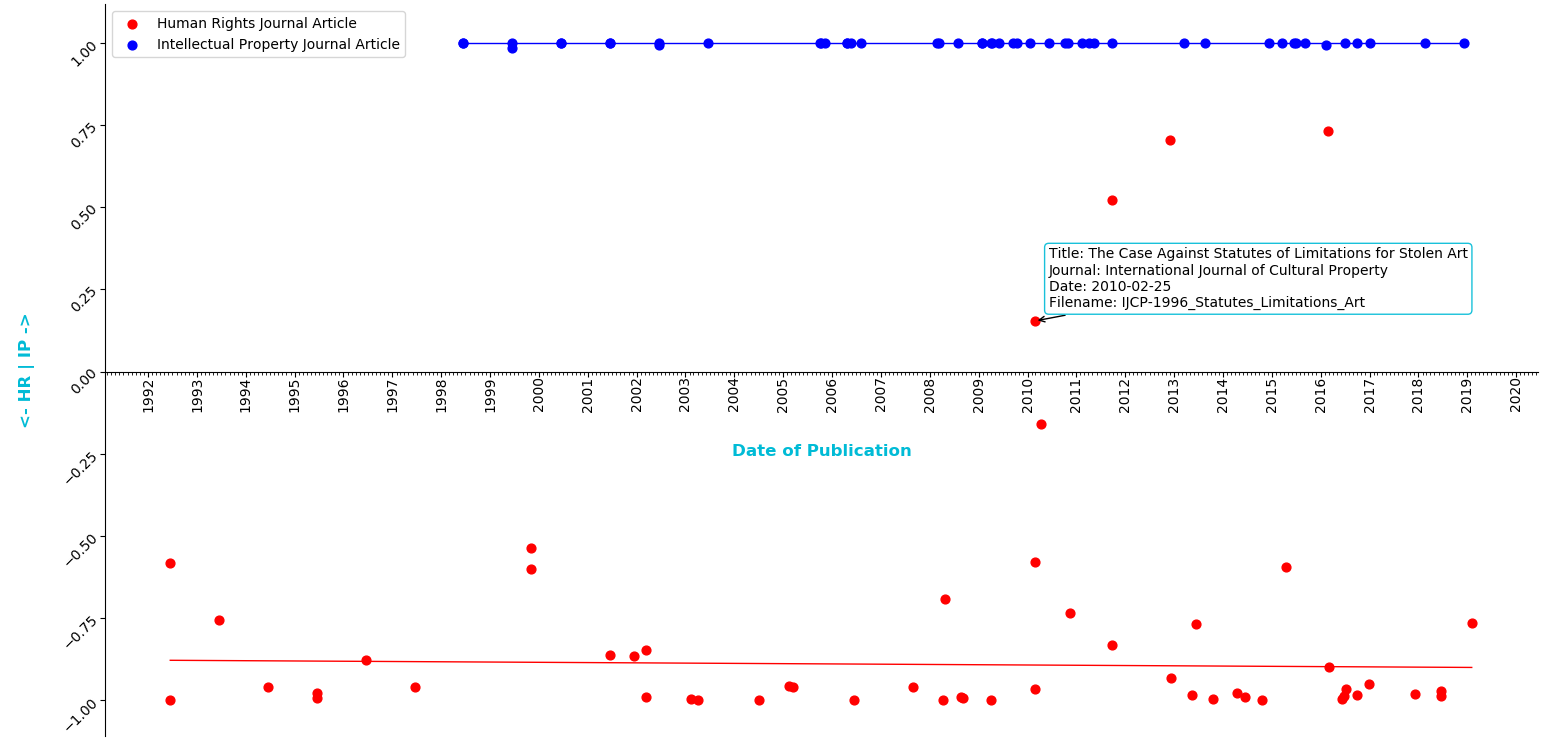
\includegraphics[width=0.9\linewidth]{resources/images/anomaly.png}
    			\caption{An annotation prompted by clicking a point.}
    			\label{fig:anomaly}
			\end{figure}
			
		\subsection{3D Enclosure}
			Since Dr. Blakely originally stated her request for a 3D visualisation, I attempted for that to carry some of the same advantages that the 2D visualisations have. I particularly wanted the same use of enclosure by the axes to indicate the predicted class that was used for the 2D visualisations. However, it is not possible to move a set of 3Daxes to the inside of a visualisation. As an alternative, I plotted two surfaces. One surface extended across the plane where $y$ equals zero; this split the documents that were predicted to be classed as user benefiting as opposed to creator benefiting. The other surface extended across the plane where $x$ equals zero; this split the documents that were predicted to be classed as human rights based as opposed to intellectual property based. 
			
			I then proposed that the surfaces could be a cleaner way of solving the problem of axes polarity discussed in Subsection \ref{sec:lab} by colouring the surface with a colour map and attaching a colour bar to explain what the colours mean. This is shown in Figure \ref{fig:3d-planes} where the z-axis varies by colour. I did not manage to get both axes to vary with colour so a mixture of solutions is used here. Having used colour for the predicted classifications, I now deemed it to be a cause of confusion to also use colour for the true classifications. I instead used another preattentive feature, shape, to distinguish documents that came from human rights and intellectual property journals. In this case, circles that were above the orange plane were wrongly classified. I decided not to opt with this visualisation because there is too much going on to process easily.
			\begin{figure}
    			\centering
    			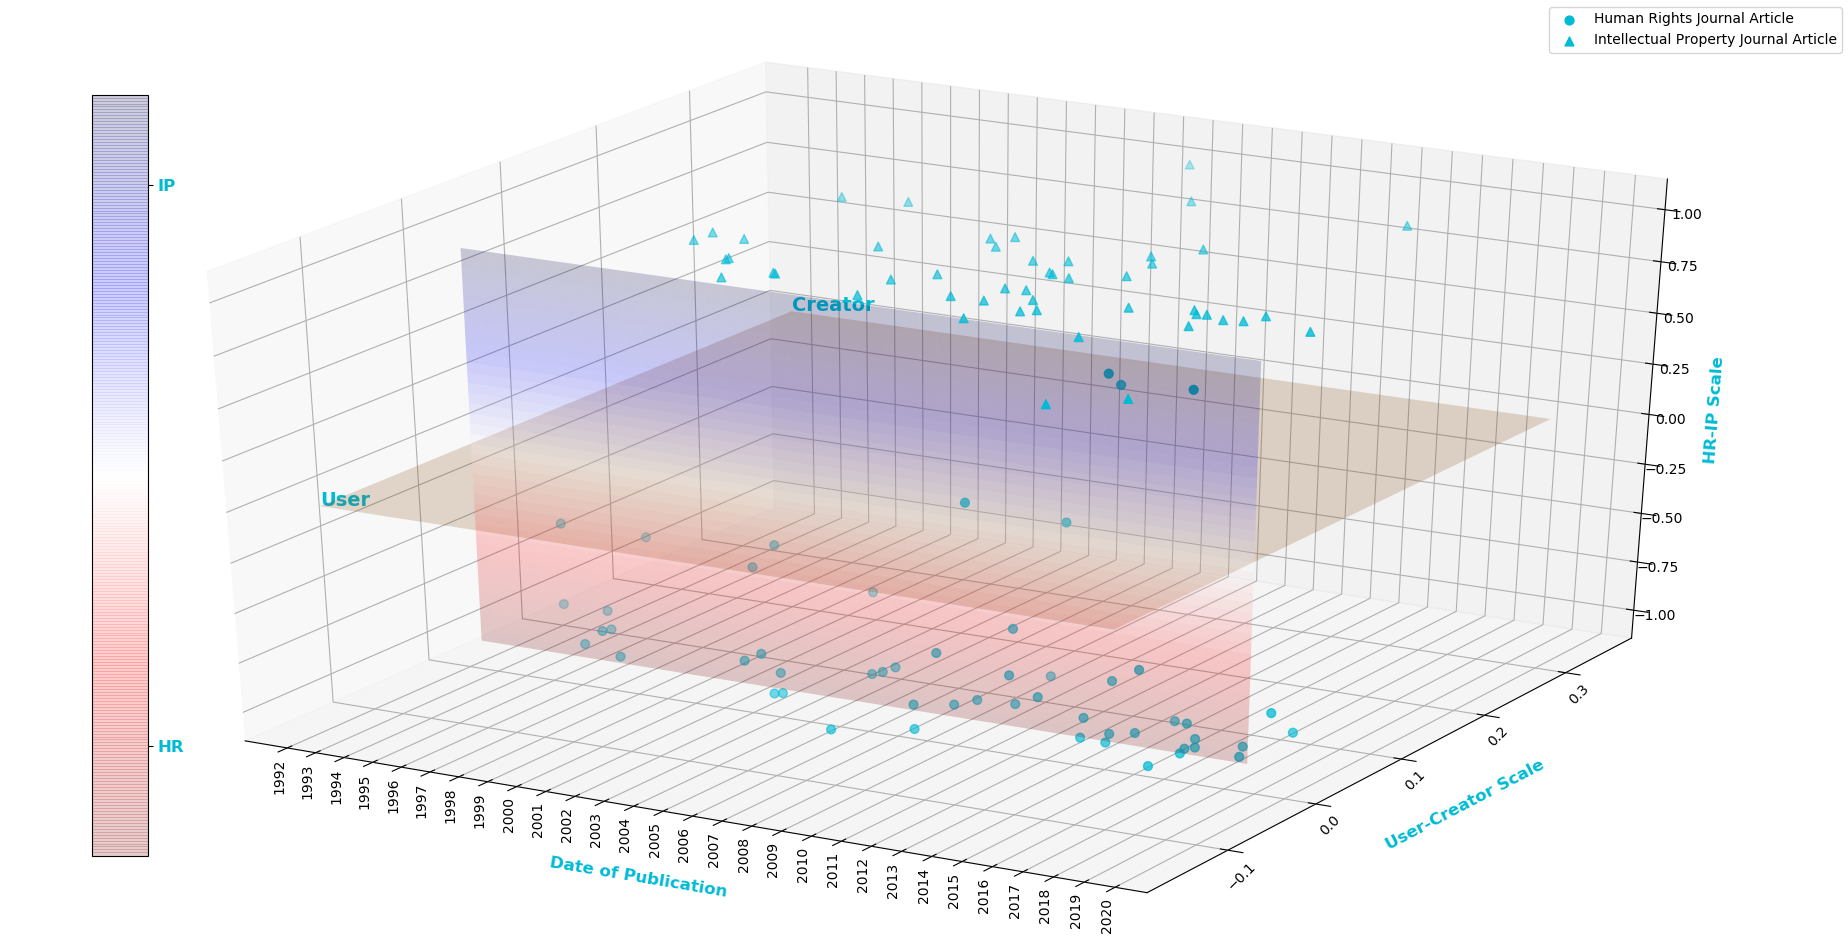
\includegraphics[width=0.9\linewidth]{resources/images/3d_planes.png}
    			\caption{A 3D visualisation with planes dividing predicted classifications.}
    			\label{fig:3d-planes}
			\end{figure}
			
	\section{Usability}
		\subsection{User Interface}\label{sec:uiimp}
			\subsubsection{Motivation}
				Much of the testing and developing was performed on a Linux terminal. This is unsuitable for the final product as most law academics do not have Linux and are not used to a terminal-based environment. This is why a graphical user interface must be made which can be booted from a desktop. The user interface must maximise the amount of time spent on analysis of results by allowing intuitive access to all features.
			\subsubsection{Executable}
				As the intended users are not used to a terminal environment, nor will they have Python installed, I used the `PyInstaller' library to create an executable for the tool meaning that they do not have to install anything extra to run the program, just the data files and the executable. This saves significant time as the user does not have to learn any complicated computer science techniques. I prioritised Windows for the executable as every academic should have some access to this operating system through their university.
			\subsubsection{Functionality}
				The user interface allows the user to view visualisations and their results with ease. It also allows them to cross-validate results via a button. The most useful functionality is regarding the documents. The user can edit the metadata in the user interface, including the title, journal and date, in case automatic extraction was not correct. This means that they do not have to go through lengthy data files for this. They can also add new documents and remove documents as well as selecting which documents are test documents. This gives them control over the input of the model so they can test article of their own interest and see where they fall on the axes. For further ease of use, there is a pop-up which allows for more options on test data and allows the user to deselect all documents as test data, select all or select a random 25\% of the documents. The user can also open PDFs directly from the user interface which is particularly useful as when the user reads the information about an anomaly in the visualisation, they do not have to leave the user interface to open the PDF and analyse the language for themselves.
				
			\subsubsection{Design}
				The user interface was programmed using Python's `Tkinter' library as it is known as the de facto standard for Python user interfaces. I started off by drawing wireframes, shown in Figure \ref{fig:ui-wire}, for Dr. Blakely's approval so I did not waste time creating a complicated user interface for it not to be suitable. I used Nielsen's heuristic of using real-world concepts by using tabs, separated by `Visualisation', `Results' and `Documents. These are clearly defined and separate sections. Dr. Blakely approved of the wireframes so I moved onto implementing them in Python.
				\begin{figure}
					\minipage{0.33\textwidth}
  						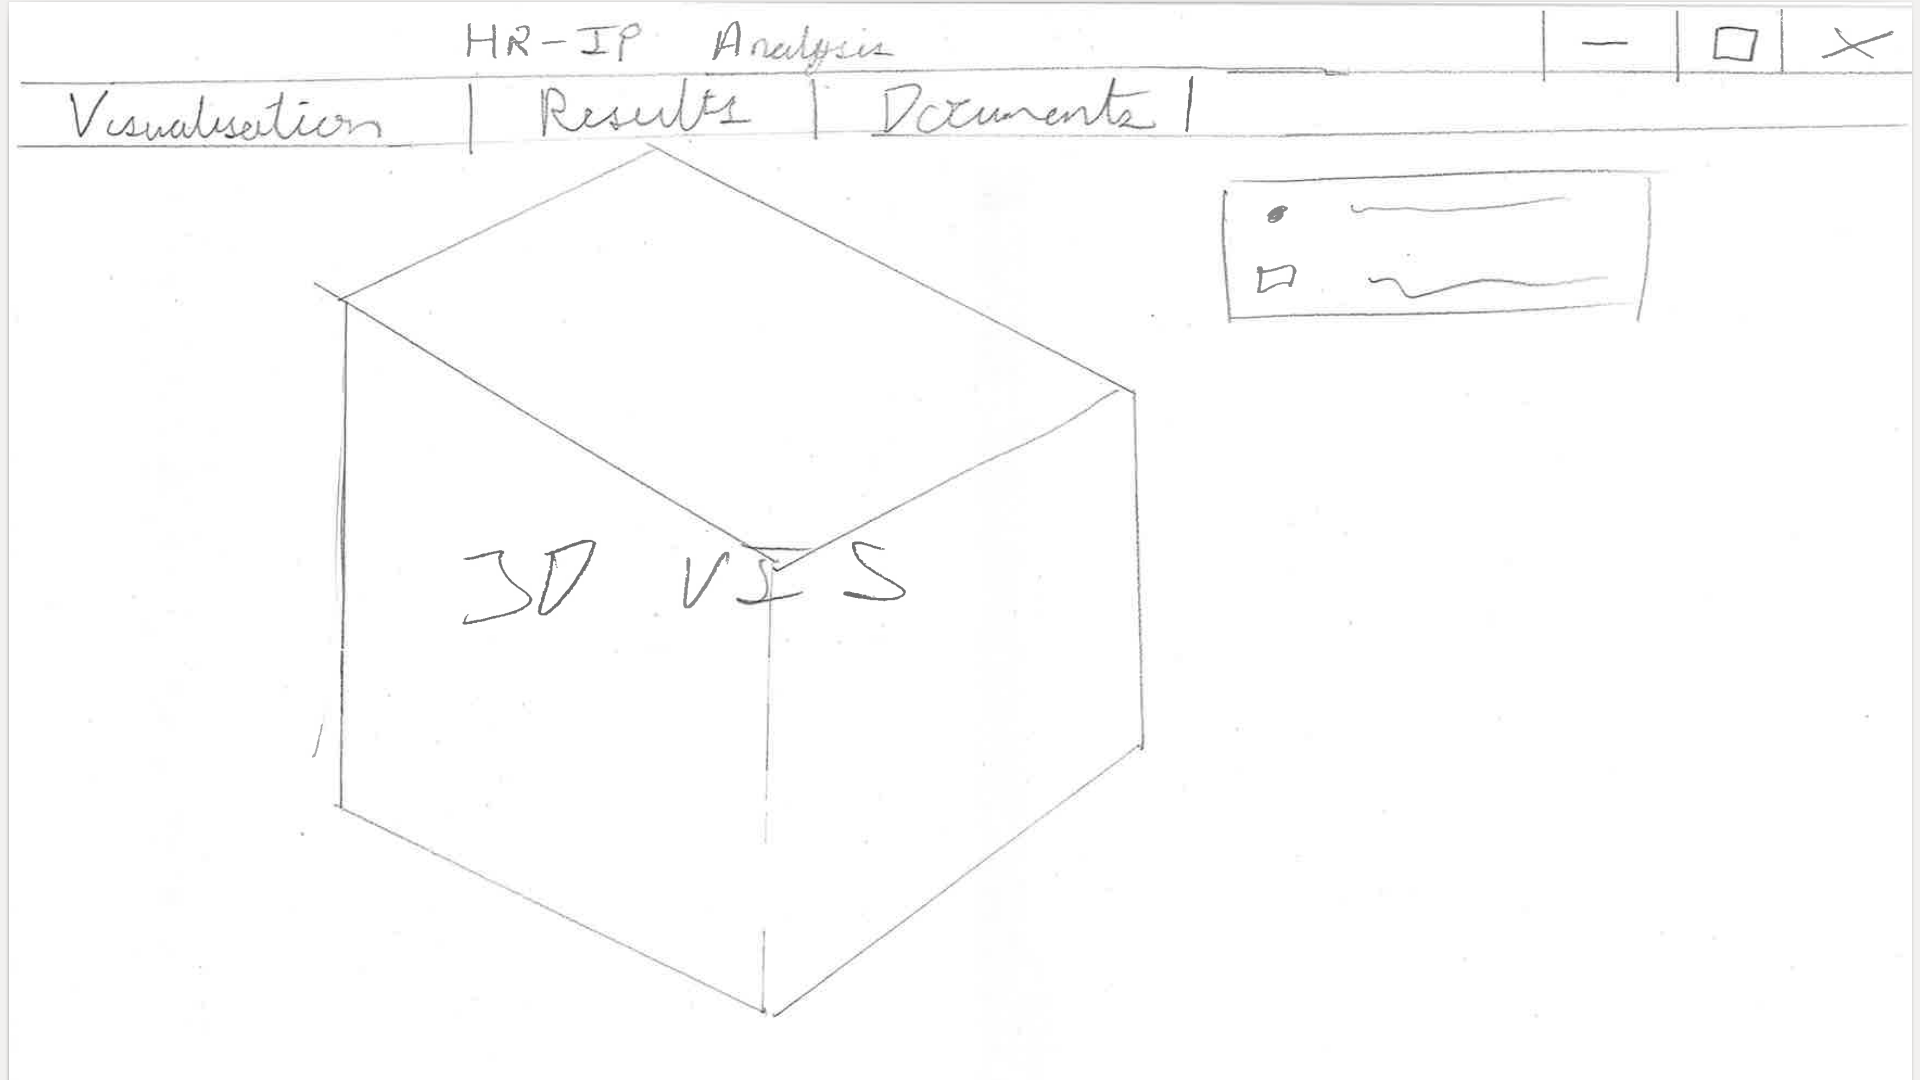
\includegraphics[width=\linewidth]{resources/images/ui_wire_3d.png}
  					\endminipage\hfill
  					\minipage{0.33\textwidth}
  						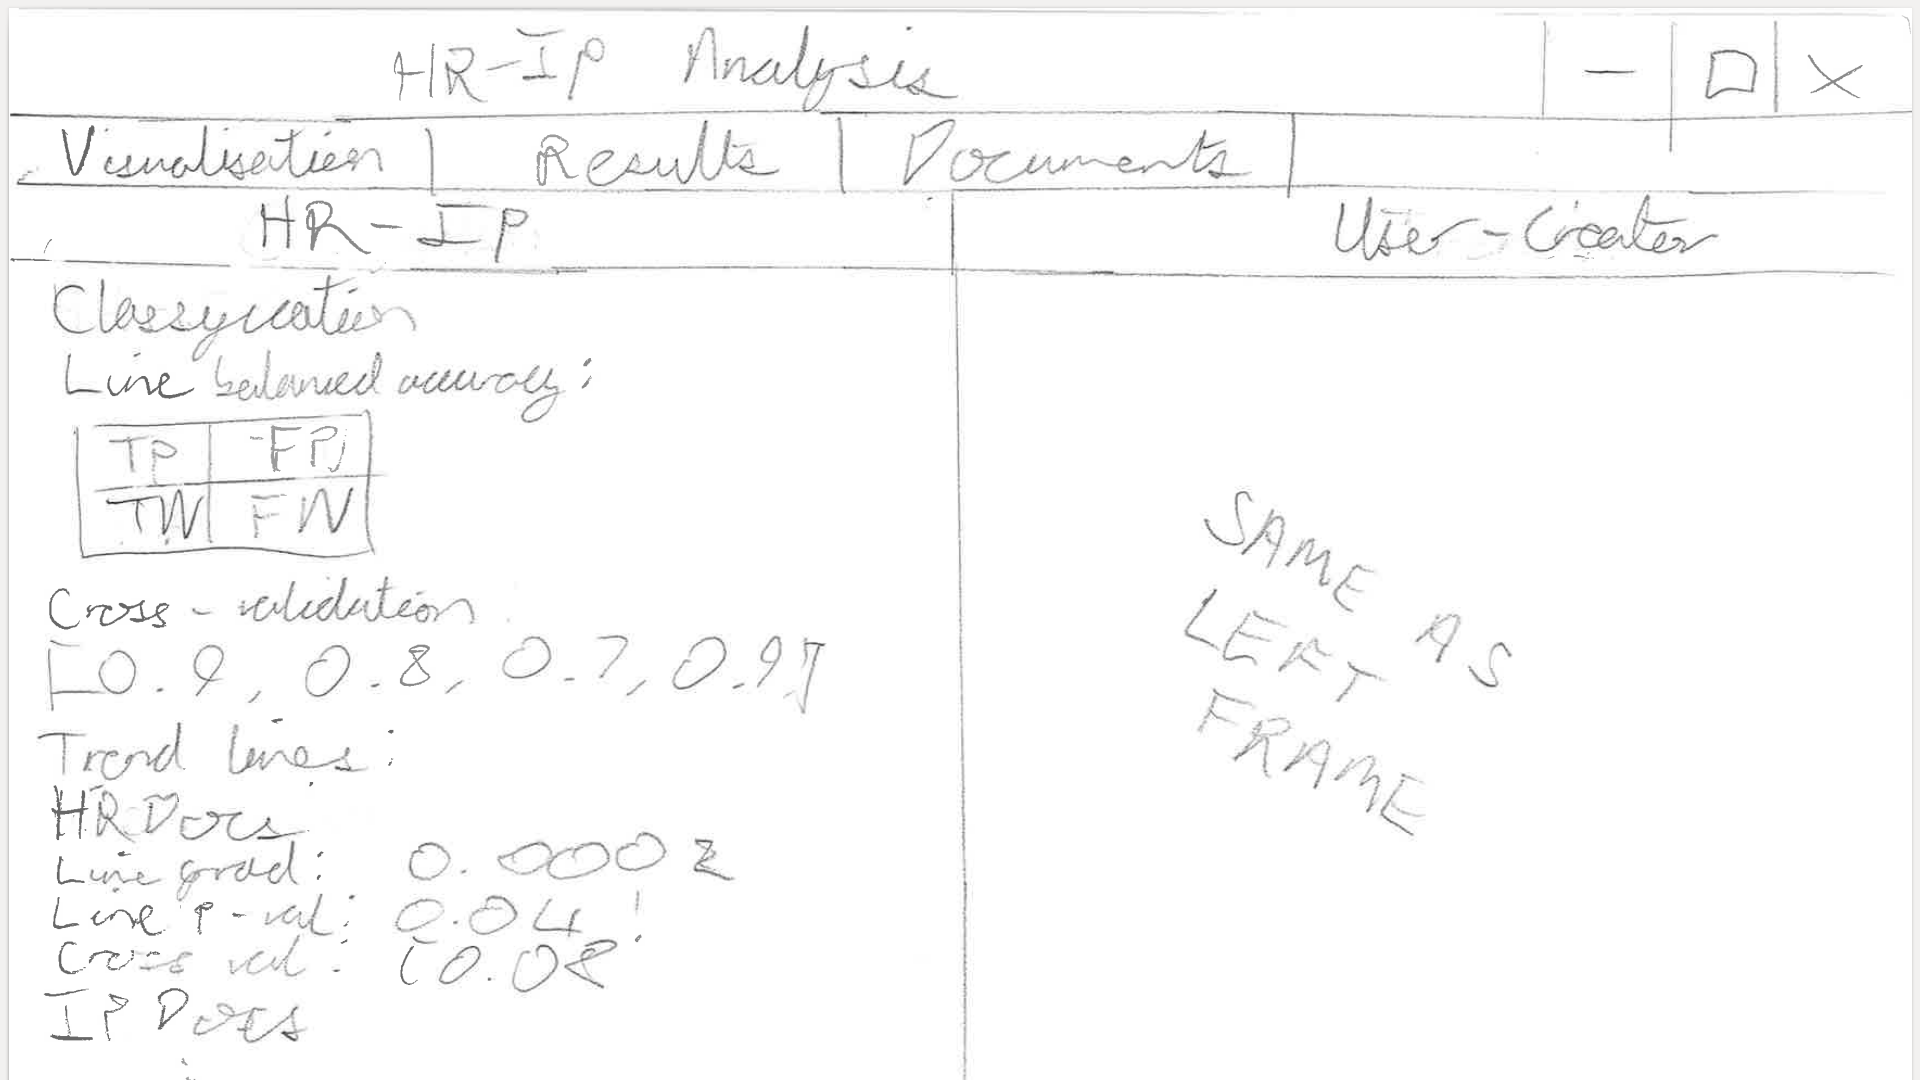
\includegraphics[width=\linewidth]{resources/images/ui_wire_eval.png}
  					\endminipage\hfill
   					\minipage{0.33\textwidth}
  						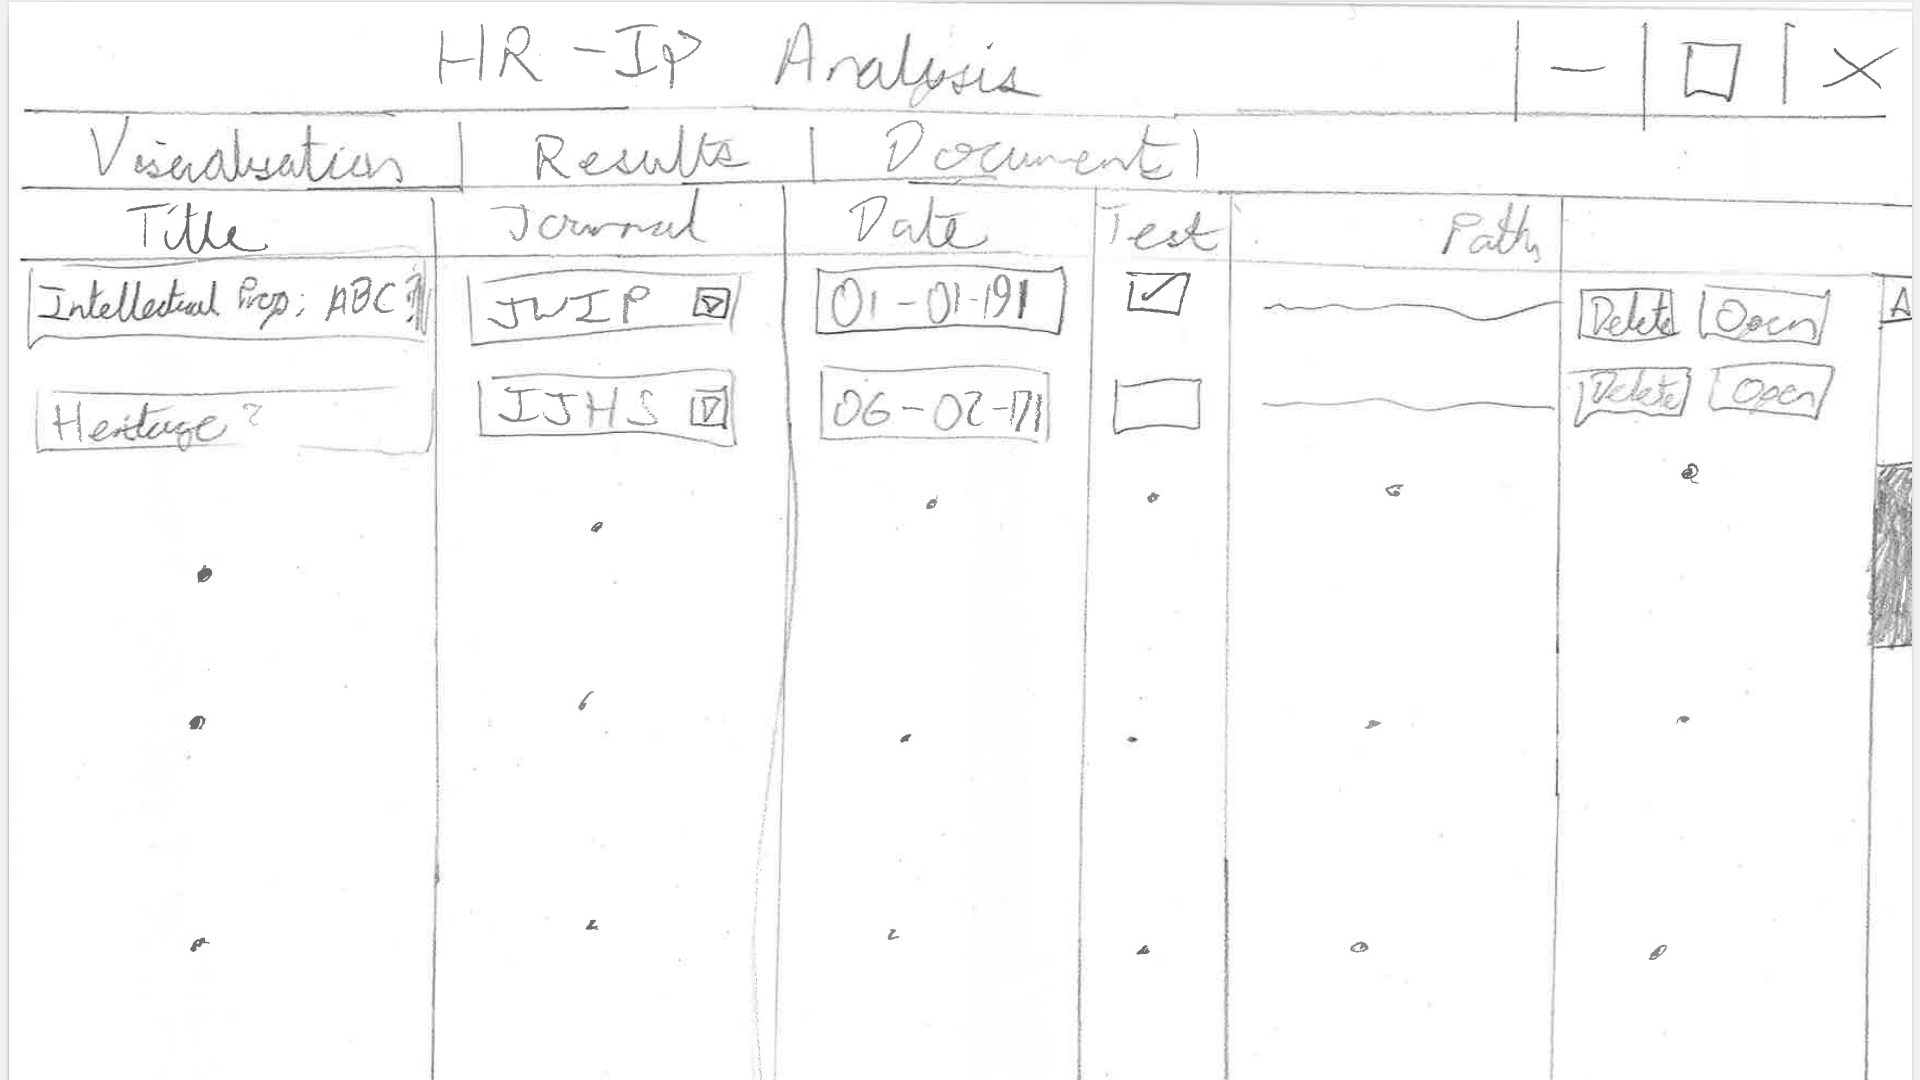
\includegraphics[width=\linewidth]{resources/images/ui_wire_documents.png}
  					\endminipage\hfill
  					\caption{Wireframes drawn for user interface.}\label{fig:ui-wire}
				\end{figure}
				
				Tabs were implemented using tkinter's `Notebook' class, the buttons' functionalities were implemented in call-back functions and the scroll bar was implemented by putting one of tkinter's `Scrollbar' objects into a `Canvas' object. The three tabs can be seen in Figures \ref{fig:ui_3d}, \ref{fig:ui_eval} and \ref{fig:ui_documents}. One notable feature is how the results for a statistically significant trend line will turn bold. This is using visualisation principles that important information should stick out via preattentive features as there is a lot of text on the screen so the important one needs attention drawn to it.
				\begin{figure}
    				\centering
    				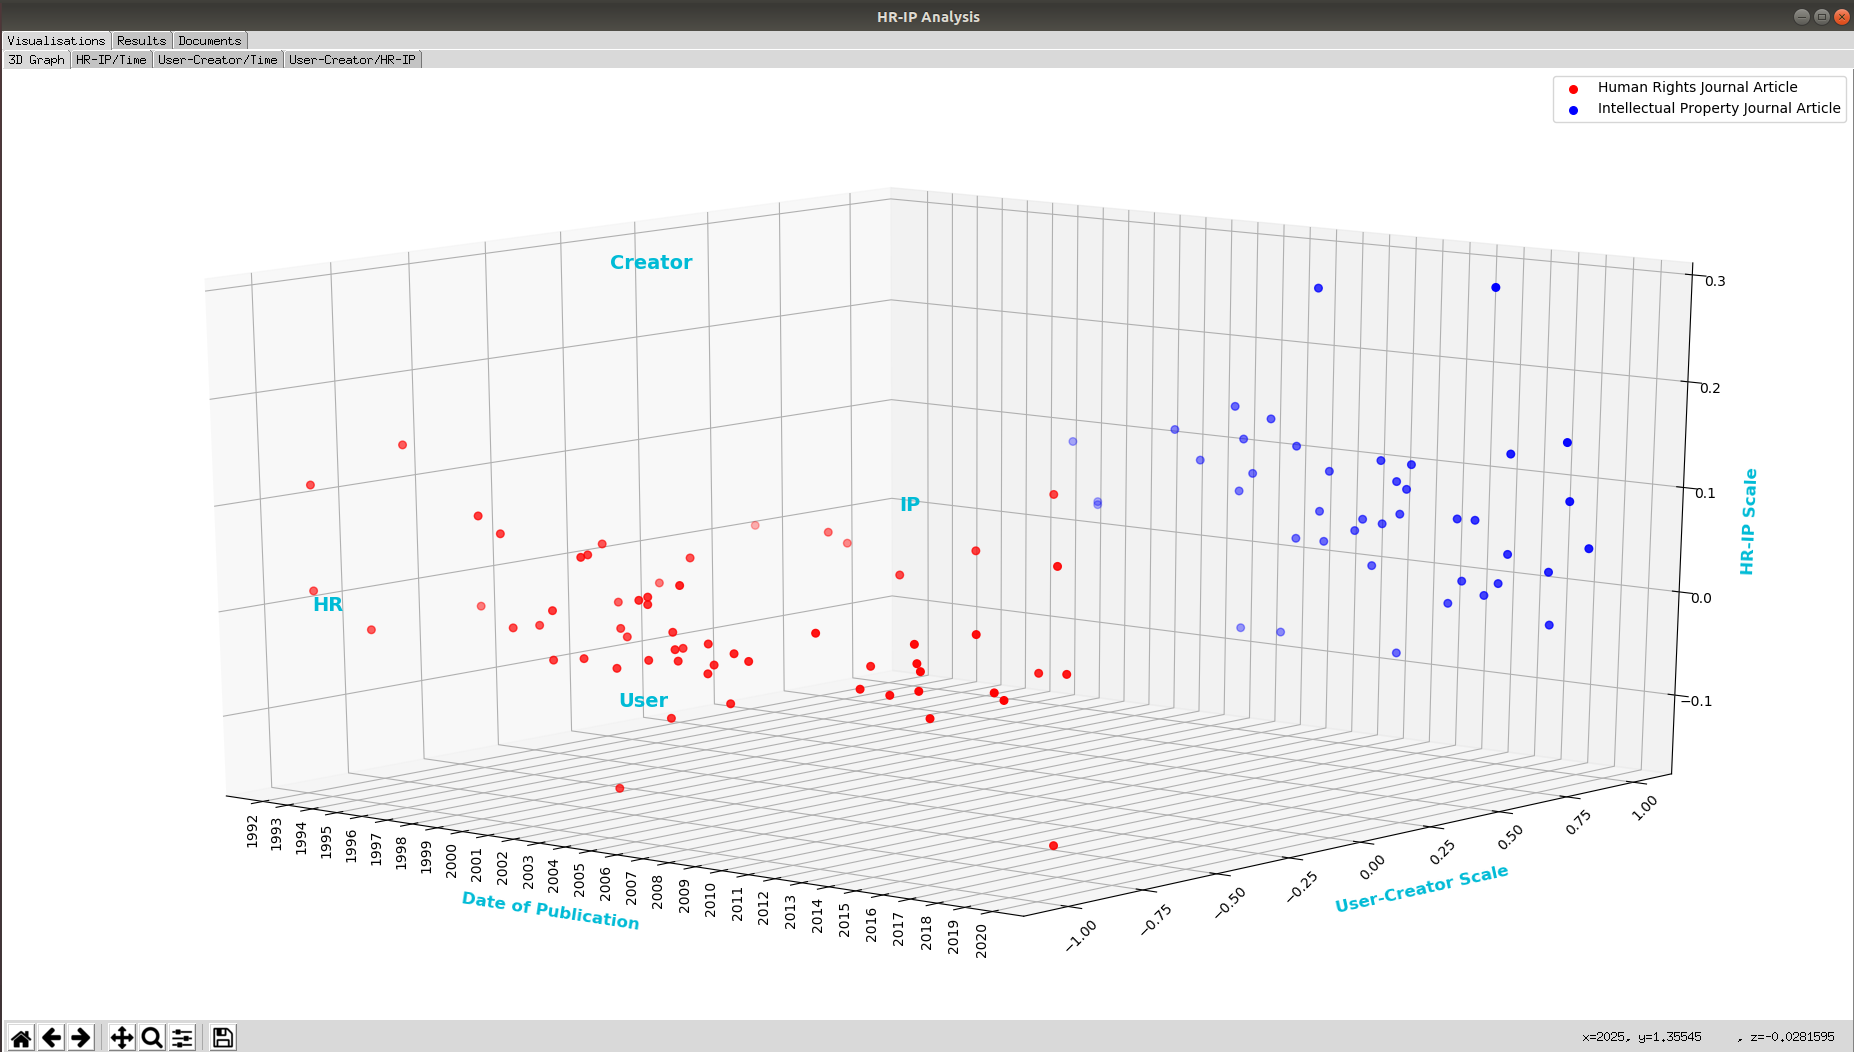
\includegraphics[width=0.9\linewidth]{resources/images/ui_3d.png}
    				\caption{The tab of the user interface displaying the 3D visualisation.}
    				\label{fig:ui_3d}
				\end{figure}
				\begin{figure}
    				\centering
    				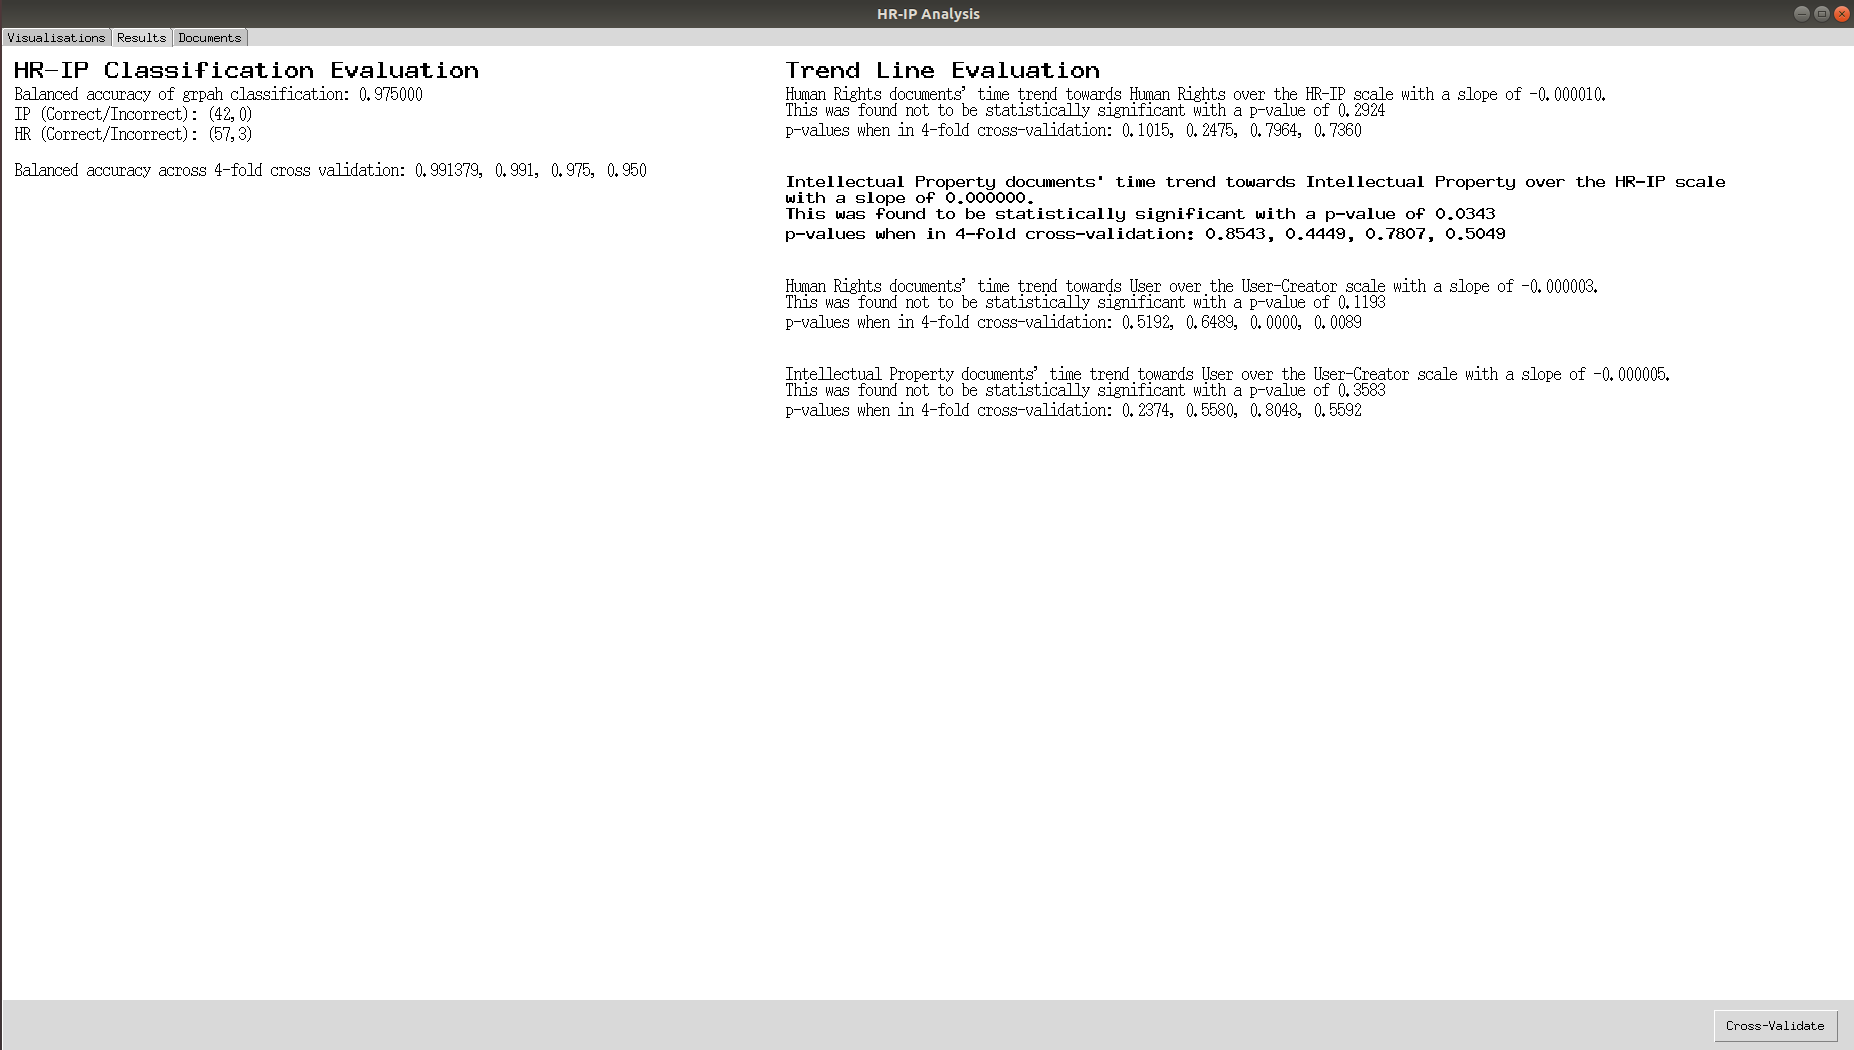
\includegraphics[width=0.9\linewidth]{resources/images/ui_eval.png}
    				\caption{The tab of the user interface displaying the evaluation data.}
    				\label{fig:ui_eval}
				\end{figure}
				\begin{figure}
    				\centering
    				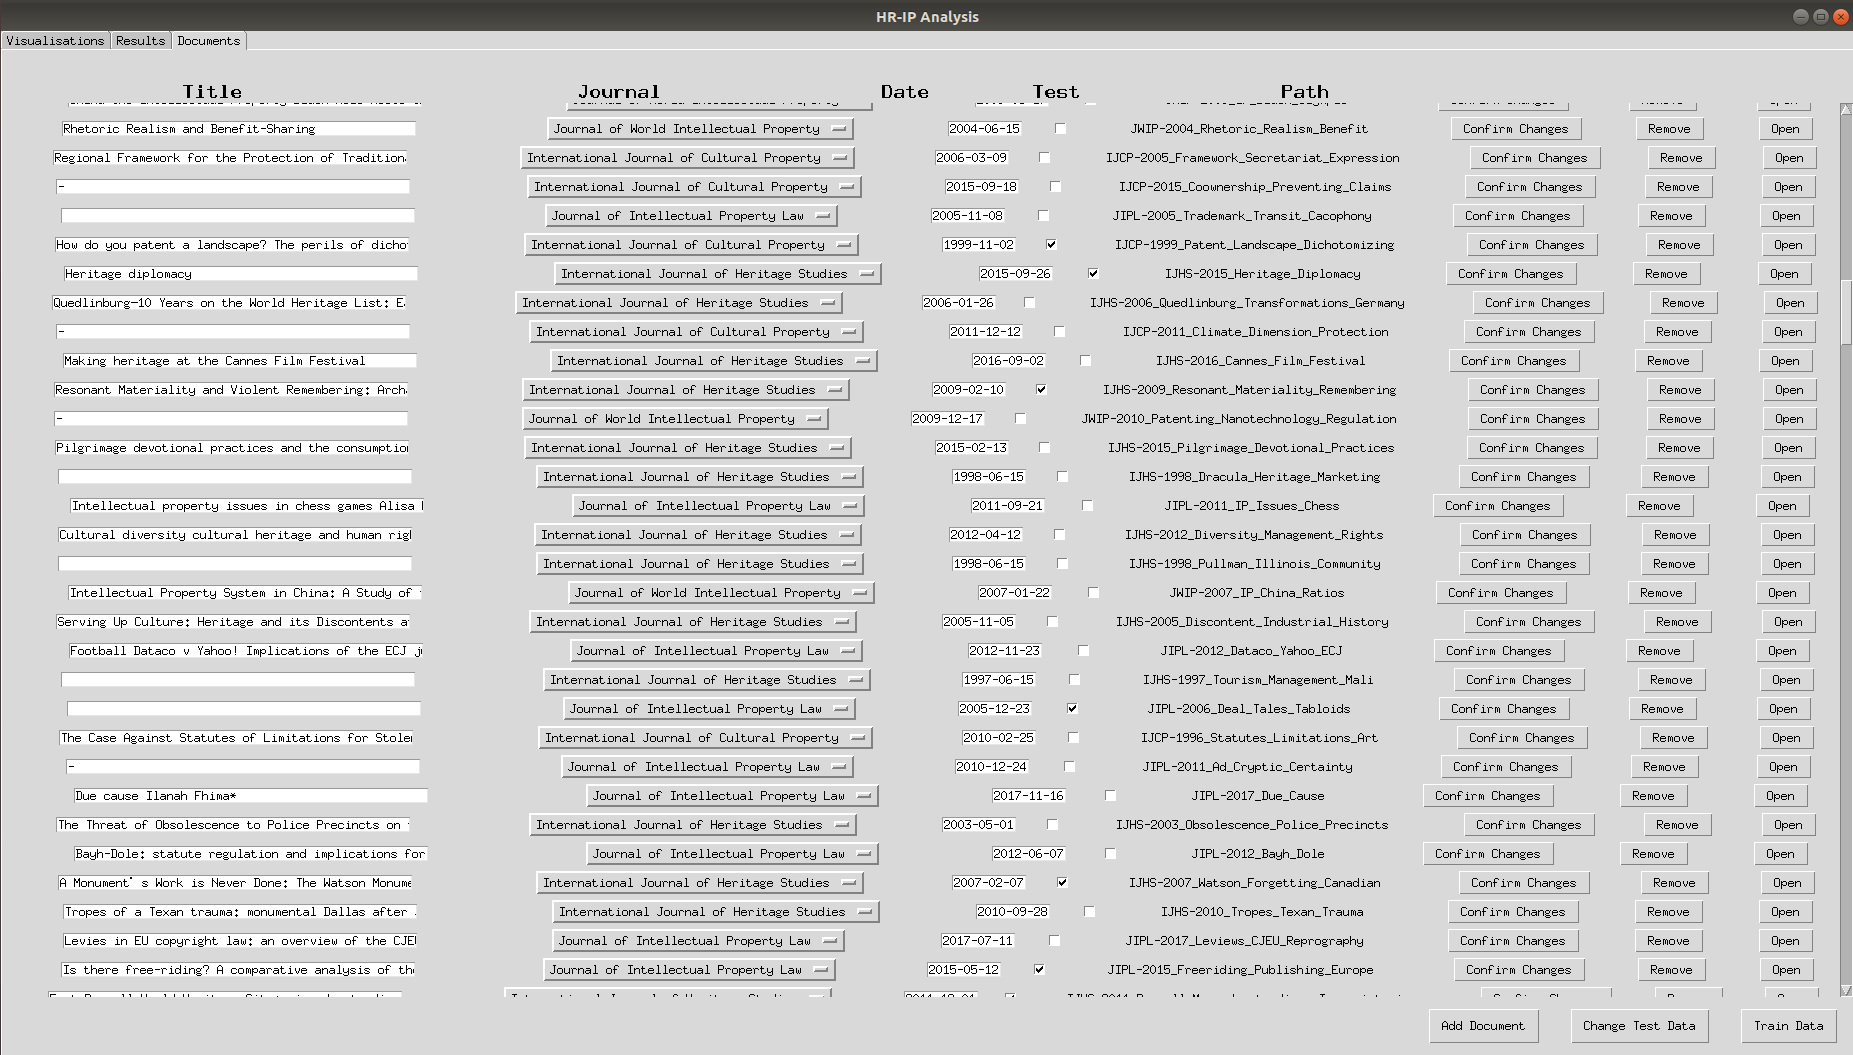
\includegraphics[width=0.9\linewidth]{resources/images/ui_documents.png}
    				\caption{The tab of the user interface displaying the list of documents used.}
    				\label{fig:ui_documents}
				\end{figure}
				
		\subsection{Speed}
			\subsubsection{Automating Metadata Assignment}
				As previously mentioned, the date an article was published, the journal it was published in and the title of the article is needed. Since a large number of documents are likely to be uploaded at once, it would be laborious to manually enter this data. For this reason, I implemented an automatic metadata extraction algorithm at the pre-processing stage. This proved to be fairly challenging due to the mixed origins of the documents.
				
				The algorithm takes the PDF of a journal article as input and outputs the article's title, journal of origin and date of first publication. A `-' as a field's output is used to indicate that the algorithm is unsure of what the field should be. This is preferred to the field being wrong since if the algorithm is correct on the first few instances, the user may assume that the algorithm is correct in all instances and not check the rest. A number of wrong fields could lead to the contamination of the training data with an incorrect ground truth assignment or the regression lines with an incorrect date assignment. 
				
				There were two means of determining the fields. The first of which was to use the PDF's metadata. This was simple to implement by using the `pdfminer' library to assign the PDF's `Creation Date' property as the date of publication and its `Title' property as its title.
				
				There are a few limitations to this method. There are no means to get the origin journal from the PDF's metadata so ground truth would have to be downloaded manually. The method is also very inconsistent. Titles are often just 'No Job Name' or 'untitled' and the `Creation Date' is often a wildly inaccurate representation of when the document was first published. This is because documents published before a certain date in each journal were not created for PDF and were scanned into PDF format later meaning their `Creation Date' was far later than their actual first publication date. If a field was empty it was marked with a `-'. The result of the algorithm over 100 samples is shown in Table \ref{tab:pdfmet}.
				
				The second means of determining the fields was to extract the information from the text. This was done by identifying different formats of documents in the dataset and identifying where each of the fields is found in each of the different formats. Regular expressions are then used, first to identify the journal and then to identify the document format. Then if the document format indicates that the PDF metadata will be correct, then the PDF metadata is used, otherwise, more regular expressions are used to identify the date and title. For example, to identify the date of publication of a document in the International Journal of Heritage Studies between 1999 and 2019, the following regular expression was used: \[[a]*\textnormal{To cite this article}[a]^*\textnormal{`}[0-9]^4\textnormal{'})\] where the single speech marks indicate the target string. 
				
				The result of this algorithm over 100 samples is shown in Table \ref{tab:textmet}. This shows that 87\% of fields are automatically filled out for the user, significantly reducing the amount of time they have to put in when inputting large numbers of documents and therefore, freeing their time to focus on analysing the results of the classification.
			\begin{table}
				\parbox{.45\linewidth}{
					\centering
					\begin{tabular}{r|c|c|c}
						\hline
						&correct&incorrect&`-'\\
						\hline
						journal&0&0&100\\
						title&25&37&38\\
						date&63&27&0
					\end{tabular}
					\caption{Success over 100 samples of determining fields using PDF method.}\label{tab:pdfmet}
				}
				\hfill
				\parbox{.45\linewidth}{
					\centering
					\begin{tabular}{r|c|c|c}
						\hline
						&correct&incorret&`-'\\
						\hline
						journal&99&0&1\\
						title&85&1&14\\
						date&77&0&23
					\end{tabular}
					\caption{Success over 100 samples of determining fields using text extraction method.}\label{tab:textmet}
				}
			\end{table}		
							
			\subsubsection{Storing Computations}
				A short way through the project, I decided to output the results of computations because the computations are repeated every time the tool is started. For example, converting all 411 PDFs to text and then counting their features takes approximately ten hours. The text only changes if the code for their conversion or cleaning changes which is rare so this does not warrant being performed every time. I found that cross-validation takes eight minutes which is too long to add to the startup time when the user may not even want to do this. They may just want to see the results of the last cross-validation. This is why the last cross-validation is stored and then loaded up on startup, rather than recomputing. This is similar to retraining and testing the data which takes approximately six minutes when it will produce the same visualisation that was previously computed. This is why all values that are plotted on the graph are stored. Considering that the loading of documents takes approximately four minutes, storing cross-validation and the plotting values rather than recomputing them means startup goes from taking 18 minutes, down to 4 minutes. Increasing the speed of startup by 78\%. This means the user does not have to remember to start the program an excessive length of time before they want to use it.
		\subsection{Codebase}
			\subsubsection{Object Orientation}
				The codebase is made refactorable by my use of object orientation. The classes are all separated clearly by their functionality. Using objects makes programming on the frontend far easier as the backend can be passed in via a single object and then navigated through via its child objects, giving it structure. An example of this is how a new tab is automatically created in the frontend for every Graph object contained in DocumentList. This means that tabs do not have to be hardcoded for every visualisation. Encapsulation is also used to avoid so it is clear where data can be manipulated from.
			\subsubsection{Commenting}
				Backend classes are commented to make the function of every class and function clear to the next developer. Some are yet to be commented but will be before handover. An example of this can be seen below:
				\begin{lstlisting}
"""
    Generates the train and test indexes for each fold of the
    cross-validation.

    Arguments:
    split             (int)
    	-- the number of folds in the cross-validation
    docsLen           (int)
        -- the total number of documents to be trained and tested
           on

    Returns:
    trainIndexesList  ([[int]])
        -- a list of lists with each list representing a different
           train and test and each integer representing the integer
           of a Document object to be trained on
    testIndexesList   ([[int]])
        -- a list of lists with each list representing a different
           train and test and each integer representing the integer
           of a Document object to be tested on
"""
				\end{lstlisting}
